%
\chapter{Theoretical foundations}
\label{cha:theor-found}
In this chapter the theoretical foundations are outlined,
providing the basic technical knowledge to undertake the project.
% 1) [X] *Project methodology: Waterfall model*
% 2) [X] *Multitasking and Pthreads*
% 3) [X] *Client-Server architecture & TCP/IP & OSI model*
% 4) [ ] /Daemons/
% 5) [ ] /Device drivers/
% 6) [ ] *Nebulizer technology for scenting*
% 7) [ ] *Gesture recognition algorithms using computer vision*
% 8) [ ] *Face detection algorithms using computer vision*
% 9) [ ] *RDBMS (Relational Database management system) (SQL)*
% 10) [ ] /User detection technologies: IR, ultrasonic/
% 11) [ ] /Camera recording and codecs/
% 12) [ ] /Image filtering APIs/
% 13) [ ] /GIFs generation/
% 14) [ ] *Social media and e-mail sharing APIs*
% 15) [ ] /UI framework: Qt/
% 16) [ ] /File transfer protocols/
% 
% Legend:
% - *Ze*
% - /Hugo/

% Proj methodology
\section{Project methodology}
\label{sec:proj-meth}
In this section the project methodologies tools are outlined, easing the
development process.

\subsection{Waterfall model}
\label{sec:waterfall-model}
For the domain-specific design of software the waterfall methodology is used.
The waterfall model (fig.~\ref{fig:waterfall}) represents the first effort to
conveniently tackle the increasing complexity in the software development
process, being credited to Royce, in 1970, the first formal description of the
model, even though he did not coin the term~\cite{sommerville1996software}. It
envisions the optimal method
as a linear sequence of phases, starting from requirement elicitation to system
testing and product shipment~\cite{cusumano1995beyond} with the process flowing
from the top to the bottom, like a cascading waterfall.

In general, the phase sequence is as follows: analysis, design, implementation,
verification and maintenance.
\begin{enumerate}
  \item Firstly, the project requirements are elicited, identifying the key
    requirements and constraints the system being developed must meet from the
    end-user perspective, captured in natural language in a product requirements document.
  \item In the analysis phase, the developer should convert the application
    level knowledge, enlisted as requirements, to the solution domain knowledge
    resulting in analysis models, schema and business rules.
  \item In the design phase, a thorough specification is written allowing the
    transition to the implementation phase, yielding the decomposition in
    subsystems and the software architecture of the system. 
  \item In the implementation stage, the system is developed, following the
    specification, resulting in the source code.
  \item Next, after system assembly and integration, a verification phase occurs
    and system tests are performed, with the systematic discovery and debugging
    of defects.
  \item Lastly, the system becomes a product and, after deployment, the
    maintenance phase start, during the product life time.
\end{enumerate}
While this cycle occurs, several transitions between multiple phases might
happen, since an incomplete specification or new knowledge about the system,
might result in the need to rethink the document.

The advantages of the waterfall model are: it is simple and easy to understand
and use and the phases do not overlap; they are completed sequentially. However,
it presents some drawbacks namely: difficulty to tackle change and high
complexity and the high amounts of risk and uncertainty. However, in the present
work, due to its simplicity, the waterfall model proves its usefulness and will
be used along the project.

As a reference in the sequence of phases and the expected outcomes from each
one, it will be used the chain of development activities and their products
depicted in fig.~\ref{fig:sw-devel-activities} (withdrawn from
\cite{bruegge2004object}).

\begin{figure}[!hbt]
\centering
    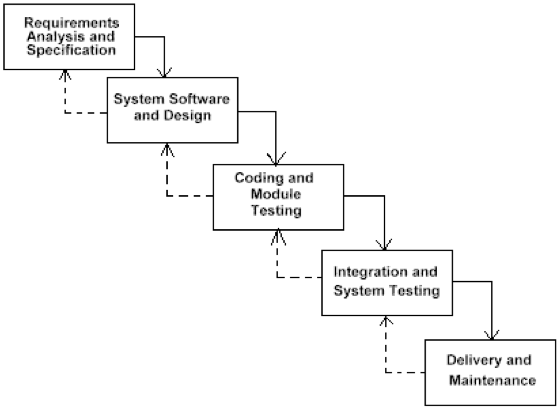
\includegraphics[width=0.6\textwidth]{./img/waterfall.png}
  \caption{Waterfall model diagram}\label{fig:waterfall}
\end{figure}

\subsection{Unified Modeling Language (UML)}
\label{subsec:uml}
To aid the software development process, a notation is required, to articulate
complex ideas succinctly and precisely. The notation chosen was the \gls{uml},
as it provides a spectrum of notations for representing different aspects of a
system and has been accepted as a standard notation in the software
industry~\cite{bruegge2004object}.

The goal of UML is to provide a standard notation that can be used by all
object- oriented methods and to select and integrate the best elements of
precursor software notations, namely \gls{omt}, Booch, and \gls{oose}
~\cite{bruegge2004object}. It provides
constructs for a broad range of systems and activities (e.g., distributed
systems, analysis, system design, deployment). System development focuses on
three different models of the system
(fig.~\ref{fig:sw-devel-activities})~\cite{bruegge2004object}:
\begin{enumerate}
  \item \textbf{\emph{The functional model}}: represented in UML with use case
    diagrams, describes the functionality of the system from the user's point of
    view.
  \item \textbf{\emph{The object model}}: represented in UML with class
    diagrams, describes the structure of the system in terms of objects,
    attributes, associations, and operations.  
  \item \textbf{\emph{The dynamic model}}: represented in UML with interaction
    diagrams, state-machine diagrams, and activity diagrams, describes the
    internal behaviour of the system.
\end{enumerate}

\begin{figure}[!hbt]
\centering
    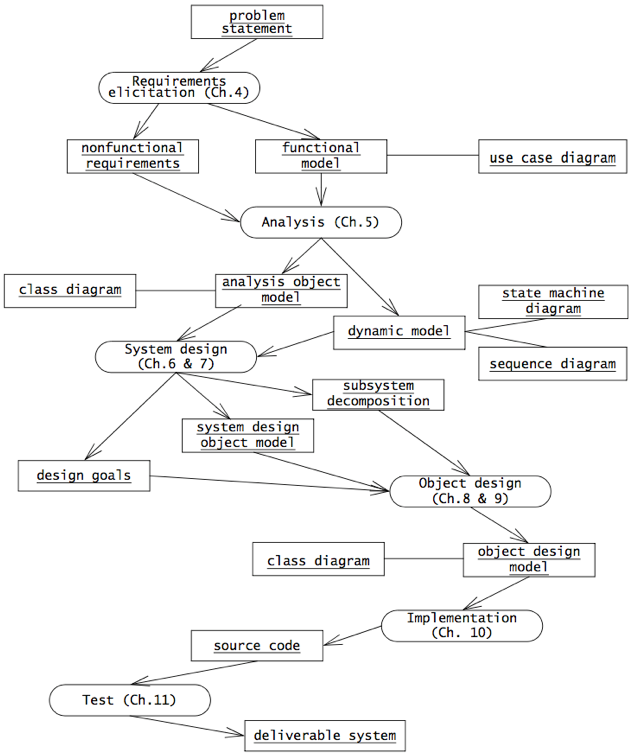
\includegraphics[width=0.7\textwidth]{./img/sw-devel-activities.png}
  \caption{An overview of the object-oriented software engineering development
  and their products. This diagram depicts only logical dependencies among work
  products (withdrawn from~\cite{bruegge2004object})}
\label{fig:sw-devel-activities}
\end{figure}

%%% Local Variables:
%%% mode: latex
%%% TeX-master: "../../../dissertation"
%%% End:

% multitask
%
\section{Multitasking and concurrency}
\label{sec:mult-conc}
aaaaaaaa

\subsection{Pthreads}
\label{sec:pthreads}
aaaaaaaa





%%% Local Variables:
%%% mode: latex
%%% TeX-master: "../../../dissertation"
%%% End:

% cli-serv
%
\section{Communications}
\label{sec:comm}
The communications technologies and the associated tools used for the project development are briefly described next.

\subsection{IEEE 802.11 --- Wi-Fi}%
\label{sec:wifi}
IEEE 802.11, commonly known as Wi-Fi, is part of the IEEE 802 set of \gls{lan} protocols, and specifies the set of \gls{mac2} and
physical layer protocols for implementing \gls{wlan}
communication in a wide sprectrum of frequencies, ranging from 2.4--60 GHz.

\subsubsection{TCP/IP}%
\label{sec:tcpip}
The most commonly used protocols for Internet communications, including Wi-Fi,
are \gls{tcp} and \gls{ip}, usually associated together, being part of the \gls{osi} model
(Fig.~\ref{fig:osi-model}), which characterises and standardises the
communication functions of a telecommunication or computing system, being
agnostic to their underlying internal structure and technology.

A computer protocol is a standardised procedure for the exchange and
transmission of data between devices, as requested for the application processes.
The TCP provides services at the Transport layer, handling the reliable, unduplicated
and sequenced delivery of data~\cite{carne2004professional}, while the UDP provides data transportation
without guaranteed data delivery or acknowledgments. The TCP can be thought of
a reliable version of \gls{udp}, generalizing. The IP part of the TCP/IP suite, providing
services at the Network layer, is used to make origin and destination addresses
available to route data across networks.

These protocols are applied in sequence to the user's data to create a frame
that can be transmitted from the sending application to the receiving
application.
The receiver reverses the procedure to obtain the original user’s data and pass
them to the receiving application~\cite{carne2004professional}.

Another interesting fact, due to the technology agnostic aspect of the OSI
Model, is that IP and the higher-level protocols may be implemented on several
kinds of physical nets.
% OSI model
\begin{figure}[!hbt]
\centering
    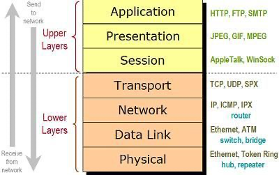
\includegraphics[width=0.5\textwidth]{./img/osi-model.png}
  \caption{\gls{osi} model}%
\label{fig:osi-model}
\end{figure}
%
\subsection{Network programming --- sockets}%
\label{sec:netw-progr-sock}
Computer systems implement multiple processes which require an identifier. As
such, the IP address is not enough to uniquely identify the origin/destination
of data to be transmitted, and the port number is added. This combination of an
IP address and port number is sometimes called a network socket~\cite{wright1995tcp}, allowing
data to be delivered to multiple processes in the same machine --- same IP
address.
It is the socket pair (the 4-tuple consisting of the client IP address, client
port number, server IP address, and server port number) that specifies the two
end points that uniquely identifies each TCP connection in an
internet~\cite{wright1995tcp}. 

In a broader sense, a socket can be described as a method of \gls{ipc} that allows data to be exchanged between applications, either on
the same host (computer) or on different hosts connected by a network~\cite{kerrisk2010linux}, as a
local interface to a system, created by the applications and controlled by the
operating system, allowing an application process to simultaneously send and
receive messages from other processes.

The Socket API was created in UNIX BSD 4.1 in 1981, with widespread
implementation in UNIX BSD 4.2~\cite{kerrisk2010linux}. It implements the Client-Server paradigm and
implement several (standard) functions to access the operating system network
resources, through system calls, in Linux~\cite{kerrisk2010linux}.

There are two generic ways to use sockets: for outgoing connections --- client
socket --- and for incoming connections --- server
socket. Fig.~\ref{fig:sockets-connection} illustrates the required steps to
obtain a connected socket:
\begin{enum-c}
\item When a socket is initially created is mostly unuseful.
\item Binding the server socket associates it to an unique network tuple (address and
  port number), enabling it to be uniquely addressed.
\item When a socket server goes into listening mode, the remote devices can
  initiate the connection procedure, referring to its unique network tuple.
\item When the socket server accepts a connection, it spawns a new socket which
  is connected to the remote device, and the endpoints can effectively
  communicate. The server socket is ready to accept new incomming connections.
\end{enum-c}
% Sockets connection
\begin{figure}[!hbt]
\centering
    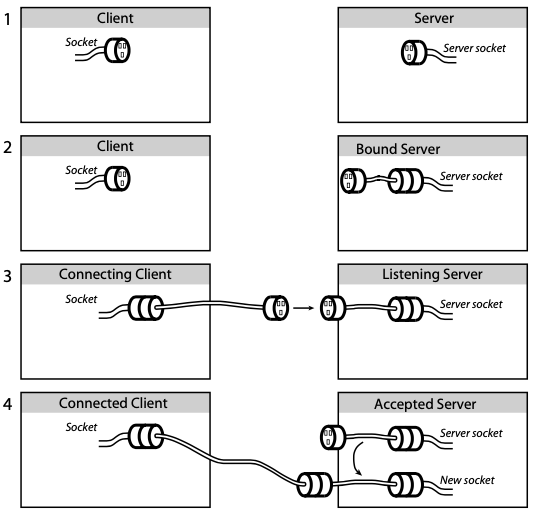
\includegraphics[width=0.6\textwidth]{./img/sockets-connection.png}
  \caption{Steps to obtain a connected socket (withdrawn from~\cite{huang2007bluetooth})}%
\label{fig:sockets-connection}
\end{figure}

\subsection{Client/server model}%
\label{sec:client-serv-model}
The client/server model is the most common form of network architecture used
in data communications today~\cite{hanson2000client}. A client is a system or
application that request the activity of a service provider system or
application, called servers, to accomplish specific tasks.
The client/server concept functionally divides the execution of a unit
of work between activities initiated by the end user (client) and resource responses
(services) to the activity request as a cooperative environment~\cite{hanson2000client}. The client,
typically handling user interactions and data exchange/modification in the user’s
behalf, makes a request for a service, and a server, often requiring some resource
management (synchronization and access to the resource), performs that service,
responding to the client requests with either data or status information~\cite{ibmCliServ}.

An example of a simple client-server model using the Socket \gls{api}, through system
calls, is presented in Fig.~\ref{fig:cli-serv-operation}. The operation of sockets can be explained as
follows~\cite{kerrisk2010linux}:
\begin{itemize}
\item The \texttt{socket()} system call creates a new socket, establishing the
  protocols under which they should communicate. For both client and server to
communicate, each of them must create a socket.
\item  Communication via a stream socket is analogous to a telephone call. One
application must connect its socket to another application’s socket before
communication can take place. Two sockets are connected as follows:
\begin{enumerate}
\item One application, assuming the role of server, calls \texttt{bind()} to
  bind the socket to a well-known address, and then calls \texttt{listen()} to
  notify the kernel it is ready to accept incoming connections.
\item The other application, assuming the role of client, establishes the
  connection by calling \texttt{connect()}, specifying the address of the socket
  to which the connection is to be made.
\item The server then accepts the connection using \texttt{accept()}. If the
  \texttt{accept()} is performed before the client application calls
  \texttt{connect()}, then the \texttt{accept()} blocks.
\end{enumerate}
\item Once a connection has been established, data can be transmitted in both
directions between the applications (analogous to a bidirectional telephone
conversation) until one of them closes the connection using \texttt{close()}.
\item Communication is performed using the conventional \texttt{read()} and
  \texttt{write()} system calls or via a number of socket-specific system calls
  (such as \texttt{send()} and \texttt{recv()}) that provide additional
  functionality. By default, these system calls block if the \gls{io} operation
  can’t be completed immediately. However, nonblocking \gls{io} is also
  possible.
\end{itemize}
% Overview of UNIX system calls
\begin{figure}[!hbt]
\centering
    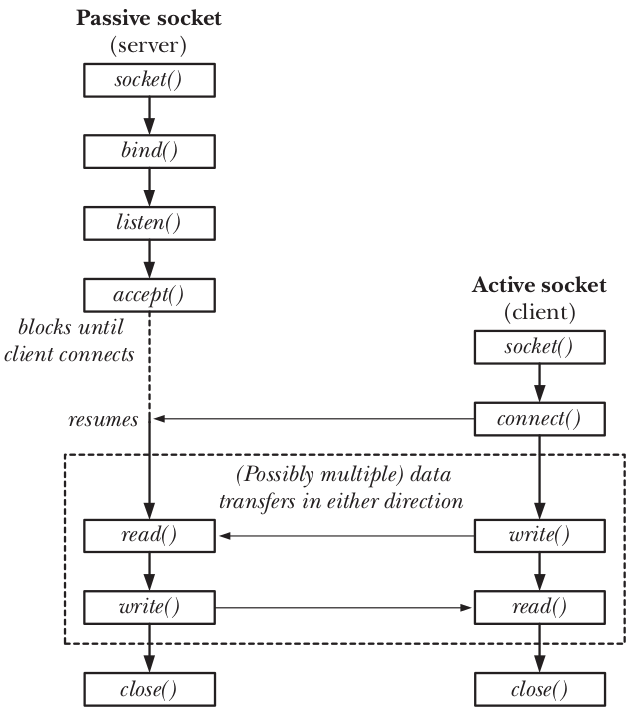
\includegraphics[width=0.62\textwidth]{./img/cli-serv-operation.png}
  \caption{Overview of UNIX system calls with sockets implementing 
a server/client paradigm (withdrawn from~\cite{kerrisk2010linux})}%
\label{fig:cli-serv-operation}
\end{figure}

%%% Local Variables:
%%% mode: latex
%%% TeX-master: "../../../dissertation"
%%% End:

% cli-serv
\section{Daemons}
\label{sec:daemons}
In this section daemons are introduced, showing how to create them, handle
possible errors and how to communicate with them.
%
\subsection{What is a Daemon?}
A daemon is a background process that runs without user input and usually provides some service, either for the system as a whole or for user programs.~\cite{daemons-slides}

Normally, daemons are started when a system boots and, unless forcibly terminated, run until system shutdown.
Because a daemon does not have a controlling terminal, any output,
either to \textit{stderr} or \textit{stdout}, requires special handling.
They often run with \texttt{superuser privilege} because they use privileges
ports (1 - 1024) or because they have access to some sort of privileged resource.
Generally, daemons are process group leaders and session leaders, a daemon's parent is the \texttt{init} process, which has the PID of 1 (daemon is an orphan process inherited by init).

\subsection{How to create a Daemon}
The steps to create a daemon are:
%
\begin{enum-c}
\item \texttt{Fork} and exit in the parent process;
\item Create a new session in the child using the \texttt{setsid} call;
\item Make the root directory, "\texttt{/}", the child process's working directory;
\item Change the child process's umask to 0;
\item Close any unneeded file descriptor the child inherited.
\end{enum-c}

\paragraph{\textbf{Fork and exit in the parent process}}
%
A daemon is started from a shell script or the command line.
Daemons are unlike application programs because they are not interactive, i.e., they run in the background and, as a result, do not have the controlling terminal.

The parent forks and exits as the first step toward getting rid of the controlling terminal (they only need a terminal interface long enough to get started).

\lstinputlisting[language=c,firstline=1, lastline=13,
caption={},
%label=lst:kf-main-short,
style=customc]{./listing/daemon_ex.c}

\paragraph{\textbf{Create a new session in the child using the setsid call}}
%
Calling \texttt{setsid} accomplishes several things:
\begin{item-c}
%
\item It creates a new session if the calling process is not a process group leader, making the calling process the session leader of the new session;
\item It makes the calling process the process group leader of the new process group;
\item It sets the \gls{pgid} and the \gls{sid} to the \gls{pid} of the calling process;
\item It dissociates the new session from any controlling \texttt{tty}.
%
\lstinputlisting[language=c,firstline=15, lastline=20,
caption={},
%label=lst:kf-main-short,
style=customc]{./listing/daemon_ex.c}
%
\item Each process is a member of a process group, which is a collection of one or more processes generally associated with each other for the purposes of job control (\textit{\# cat ship-inventory.txt | grep booty | sort}).
\item When a new user first logs into a machine, the login process creates a new session that consists of a single process, the user’s login shell. The login shell functions as the session leader.
%
\end{item-c}

\paragraph{\textbf{Make the root directory, "/", the child process's working directory}}
%
This is necessary because any process whose current directory is on a mounted file system will prevent that file system from being unmounted.

Making "/" a daemon's working directory is a safe way to avoid this possibility.
%
\lstinputlisting[language=c,firstline=22, lastline=29,
caption={},
%label=lst:kf-main-short,
style=customc]{./listing/daemon_ex.c}
%

\paragraph{\textbf{Change the child process's umask to 0}}

This step is necessary to prevent the daemon's inherited umask from interfering with the creation of files and directories.

Consider the following scenario:
\begin{item-c}
\item A daemon inherits a umask of 055, which masks out read and execute permissions for group and other. 
\item Resetting the daemon’s umask to 0 prevents such situation.
\end{item-c}
%
\lstinputlisting[language=c,firstline=31, lastline=35,
caption={},
%label=lst:kf-main-short,
style=customc]{./listing/daemon_ex.c}
%

\paragraph{\textbf{Close any unneeded file descriptor the child inherited}}
%
This is simply a common sense step. There is no reason for a child to keep open descriptors inherited from parent.
The list of potential file descriptors to close includes at least stdin, stdout and \texttt{stderr}.
%
\lstinputlisting[language=c,firstline=37, lastline=43,
caption={},
%label=lst:kf-main-short,
style=customc]{./listing/daemon_ex.c}
%

\subsection{How to handle errors}
%
There's the \textbf{problem} that once a daemon calls \texttt{setsid}, it no longer has the controlling terminal an so it has nowhere to send output that would normally go to \texttt{stdout} or \texttt{stderr} (such as error messages).

The \textbf{solution} is that, fortunately, the standard utility for this purpose is the \texttt{syslog} service, provided by the system logging daemon, \texttt{syslogd}.

\paragraph{\textbf{Handling Errors with syslog}}
%
\texttt{syslogd} is a daemon that allow to save log messages from other daemons or applications.
The relevant interface is defined in \texttt{<syslog.h>} header file.
The \gls{api} is simple, \texttt{openlog} opens the log, \texttt{syslog} writes a message to it, and
\texttt{closelog} close the log.

The function prototypes are listed here:
%
\lstinputlisting[language=c,firstline=45, lastline=49,
caption={},
%label=lst:kf-main-short,
style=customc]{./listing/daemon_ex.c}
%

\subsection{Communicating with a Daemon}
%
To communicate with a daemon, you send a it signals that cause it to respond in a given way.
For example, it is typically necessary to force a daemon to reread its configuration file.
The most common way to do this is to send a \texttt{SIGHUP} signal to the daemon.

When you execute the command \textit{"kill PID"} on command line, the signal \texttt{SIGINT} is sent to daemon to terminate the daemon execution.

%%% Local Variables:
%%% mode: latex
%%% TeX-master: "../../../dissertation"
%%% End:

% cli-serv
%
\section{Device drivers}
\label{sec:device-drivers}
aaaaaaaa


%%% Local Variables:
%%% mode: latex
%%% TeX-master: "../../../dissertation"
%%% End:

% cli-serv
%
\section{Scenting technologies}
\label{sec:scenting-techn}
A scenting technology transforms an aromatic liquid into a gaseous fluid that
can be conveyed through the air and be captured by human olfactory sense,
usually for therapeutic or marketing purposes. As aforementioned in
Section~\ref{sec:context-motivation}, olfactory sense is the fastest way to the brain, thus, providing an exceptional
opportunity for marketing~\cite{news-harvard} --- ``75\% of the emotions we generate on a daily basis are affected by smell. Next
to sight, it is the most important sense we have''~\cite{lindstrom2006brand}.

In this section a brief overview of the scenting technologies is provided, with
special focus on ultrasonic diffusion as simple to control and cost-effective
solution.

\subsection{Overview}
\label{sec:overview}
There are several scenting technologies, mainly divided into~\cite{wen2019development}:
\begin{item-c}
\item \emph{Atomization}: it dispense odorants by transforming them into a
  gaseous fluid without requiring to heat. Its advantages are
  the dispensing process is fast and the dispensing quantity is controllable.
\item \emph{Thermalization}: it dispense odorants by vaporizing odor sources in
  the liquid state of the solid state using \gls{pwm} heaters. It requires a
  temperature controller to avoid scorching odor sources.
\item \emph{Evaporation}: it dispense odorants by conveying the liquid through a
  porous material into the outer surface (capillary action) where it evaporates
  naturally. It is a passive method, thus, not controllable.
\end{item-c}

The thermalization process requires heat which can modify fragrances, besides
requiring more power. Evaporation is a passive method, hence, not
controllable. Thus, one will focus on the \textbf{atomization} processes.

There are several atomization processes, with the most commercially relevant being~\cite{aromaUltrasonicVsNebul}:
\begin{item-c}
\item \emph{Ultrasonic diffusers}: it contains reservoirs for water and
  essential aromatic oils. It uses mechanical ultrasonic vibrations to
  brake down water molecules into droplets, producing mist, diffusing the oils
  into the air. Its advantages are: low power consumption, easy to clean,
  silent operation, and
  they double as a humidifier (can be a disadvantage too). Furthermore, they are
  a very cost-effective solution: the units themselves tend to cost less than
  nebulizing diffusers on average, but more importantly, ultrasonic diffusers
  use much less oil than nebulizing diffusers. They also run for longer periods
  of time, in several cases up to 24 hours before needing to be refilled.
  As a disadvantage they change the fragrance composition by incorporating water
  into it (this is not critical).
\item \emph{Nebulizers}:
  Nebulizing diffusers don't use water. Instead the essential oil is diffused by
  an air compressor that blows air across the top of the reservoir tube,
  creating a vacuum which pulls fine particles of the essential oil up and
  sprays them into the air around the unit. Its advantages are: fragrance
  composition is unaltered, more compact (typically), faster and more
  concentrated fragrance diffusion. The drawbacks are: less cost-effective when
  compared to ultrasonic diffusers as the oil consumption rate is much higher
  and the units are more expensive, and they tend to be noisy due to the air
  compressor operation.
\end{item-c}

The ultrasonic diffuser was preferred due to its low power consumption, silent
operation, cost-effectiveness, and easy control and assembly. The ultrasonic
diffusion process will be detailed in the following section.

\subsection{Ultrasonic diffusion}
\label{sec:ultrasonic-diffusion}
Ultrasonic diffusion uses high frequency stimuli to brake down water molecules
into droplets, producing mist, diffusing the oils into the air. The high
frequency stimuli is above 20 kHz, the upper threshold
for audible human hearing --- thus the ultrasonic naming --- and it's
accomplished using micro-mesh piezoelectric transducers.

Piezoelectric transducers are reciprocating transducers as they:
\begin{item-c}
\item respond to electric stimuli by generating mechanical displacement which,
  in turn, produces waves --- \emph{inverse-piezoelectricity}.
\item respond to mechanical displacement (applied force) by generating an
  electrical voltage signal --- \emph{piezoelectricity}.
\end{item-c}

In the present case, one is more interested in the first
phenomena. Piezoelectric transducers have a ressonant frequency, which means
they will go into a natural oscillation state, amplifying oscillations. Thus,
stimulating the piezoelectric actuator with a \gls{ac} signal at the resonant
frequency produces a strong mechanical oscillation, generating waves.
For small ressonant frequencies, the liquid, e.g. water, can easily follow the
mechanical oscillation produced.
However, when the ressonant frequency is high enough (hundreds of kHz or MHz),
the water particles cannot follow the oscillating surface, thus creating
momentary vacuum, due to the negative amplitudes, which therefore creates air
bubbles.
Then, on positive amplitudes these air bubbles are pushed across the surface,
catapulting water droplets into the air, quickly dissipating and turning into
vapor form.

Fig.~\ref{fig:piezo-transducer} illustrates a type of piezoelectric transducer
for ultrasonic diffusion --- the micro-porous mesh. It is comprised of~\cite{wen2019development}:
\begin{item-c}
\item \emph{rubber gasket}: used to isolate electric conduction from other
  conducting materials and as cushion against vibration;
\item \emph{metal substrate}: it has a micro-porous metal mesh in the center
  with a high number of trumpet-shaped cylinder micro-pores, in which the upper
  cylindrical surface is smaller than the bottom.
\item \emph{ring-shaped piezoelectric plate}: a contact is attached to the
  piezoelectric plate, so that the power wire and ground wire can be connected
  between the piezoelectric plate and the metal substrate, enabling its
  electrical stimulation.
\end{item-c}
%
\begin{figure}[htb!]
\centering
    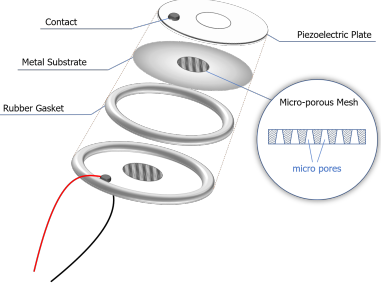
\includegraphics[width=0.55\columnwidth]{./img/piezo-transducer.png}
  \caption{Micro-porous mesh piezoelectric transducer for ultrasonic diffusion --- withdrawn from~\cite{wen2019development}}%
\label{fig:piezo-transducer}
\end{figure}

This micro-porous piezoelectric transducer is driven by an \gls{ac} signal at a
frequency of around 113 kHz and converts electric energy into kinetic energy due
to inverse-piezoelectricity~\cite{wen2019development}. The metal substrate
vibrates along with the vibration of the ring-shaped piezoelectric plate, and
the mesh in the center of the metal substrate smashes the liquid beneath the
transducer. Some liquid flows through those micro-pores and is emitted in
micro-droplet form, due to the momentary vacuum created.

The rationale behind the micro-porous piezoelectric is due to its
versatility regarding voltage supply, small size, easy control, low power
consumption and variety of fluids that it can diffuse.
A list of micro-porous piezoelectric film properties are listed below~\cite{wen2019development}:
\begin{enum-c}
\item Diameter: 13.8 mm.
\item Low driving voltage: 3--12 V.
\item High conversion efficiency, spray volume.
\item Exit aperture is very small 4 µm.
\item Frequency: 113 kHz ± 5 kHz.
\item Capacitance: 2700 PF ± 15\%.
\item Power: 1.5--2.0 W.
\item Spray volume 30 ml/h.
\item Can atomize essential oils, perfume, water based perfumes or even mixture
  of the mentioned materials.
\item life of more than 3000 hours.
\end{enum-c}

Abid et al.~\cite{abid2015novel} proposed a novel olfactory displays' scent
dispersing module based on this type of transducer
(Fig.~\ref{fig:novel-olfactory-scent-elem}). It contains a refillable fragrance
reservoir, a cotton core and the housing for the micro-porous piezoelectric
film. The fragrance ascends to the cotton core via capillary effect,
impregnating it. When the micro-porous electric film is stimulated the fragrance
in the cotton core is diffused through the aforementioned effect.
%
\begin{figure}[htb!]
\centering
    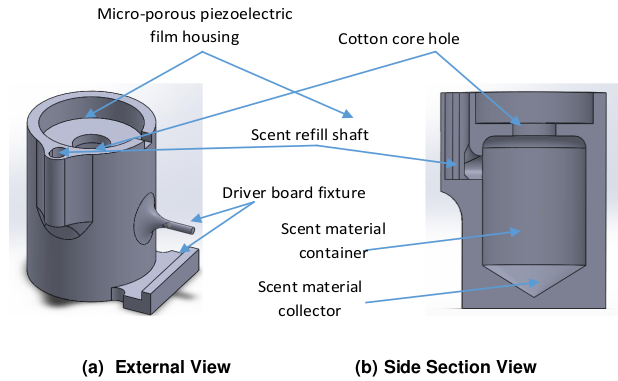
\includegraphics[width=0.65\columnwidth]{./img/novel-olfactory-scent-elem.png}
  \caption{Micro-porous mesh piezoelectric-based scent dispense module --- withdrawn from~\cite{abid2015novel}}%
\label{fig:novel-olfactory-scent-elem}
\end{figure}

\subsubsection{Driving circuit}
\label{sec:driving-circuit}
There are several commercially available \glspl{pcb} to drive micro-porous
piezoelectric transducers. Fig.~\ref{fig:pcb-diffusion} illustrates a commercial
\gls{pcb} to drive piezoelectric transducer of 113 kHz resonance frequency.
%
\begin{figure}[htb!]
\centering
    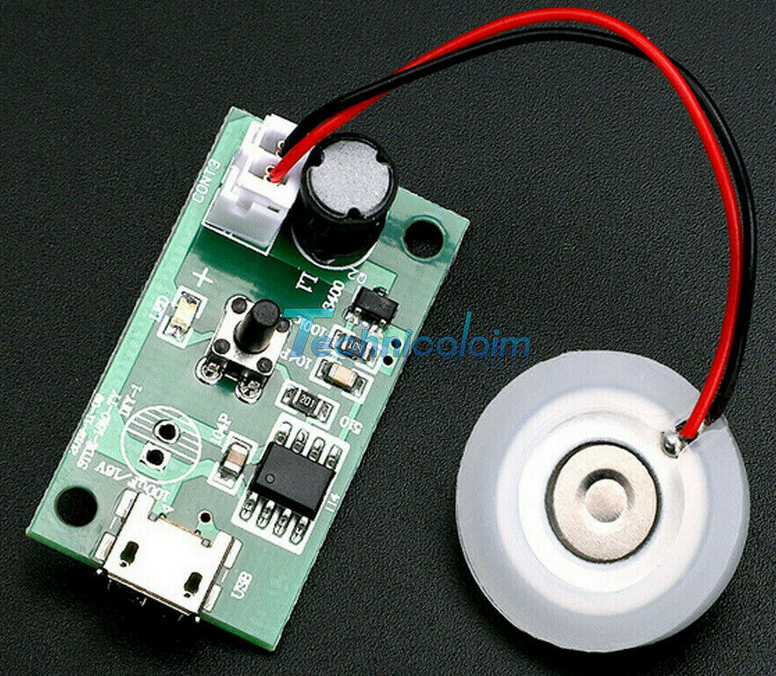
\includegraphics[width=0.4\columnwidth]{./img/pcb-diffusion.png}
  \caption{Commercial \gls{pcb} for driving micro-porous mesh piezoelectric transducers~\cite{ebayPiezo}}%
\label{fig:pcb-diffusion}
\end{figure}

As aforementioned, piezoelectric transducers for diffusion require an \gls{ac}
signal at the resonance frequency. Fig.~\ref{fig:pcb-reverse-eng} illustrates a
possible driving circuit for these transducers. A 555-timer \gls{ic} is used in
astable mode to generate a square wave at the resonance frequency that drives a
gate of power \gls{mosfet}. This \gls{mosfet} which feeds an resonant circuit to
generate an \gls{ac} signal which stimulates the piezoelectric transducer,
producing mechanical oscillations at the resonance frequency. This application
requires a fast-switching power \gls{mosfet}, like the IRLZ44N, as the
piezoelectric transducer consumes up to 300 mA of current. 
%
\begin{figure}[htb!]
\centering
    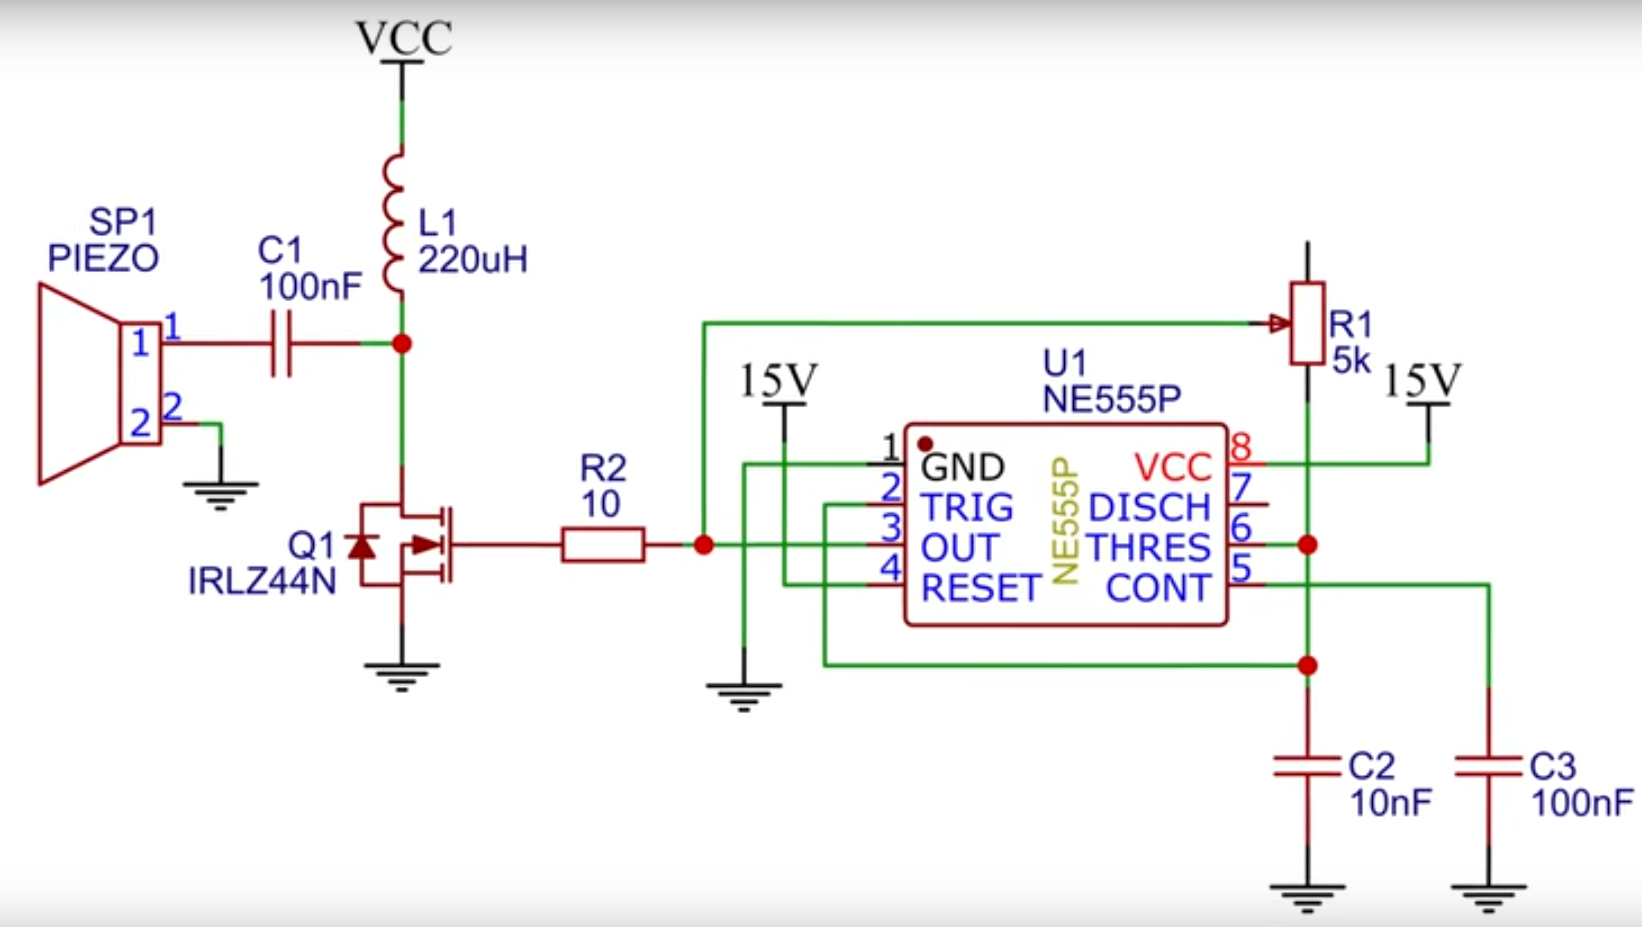
\includegraphics[width=0.6\columnwidth]{./img/pcb-reverse-eng.png}
  \caption{Schematic of a driving circuit for micro-porous mesh piezoelectric transducers~\cite{piezoSchematic}}%
\label{fig:pcb-reverse-eng}
\end{figure}



%%% Local Variables:
%%% mode: latex
%%% TeX-master: "../../../dissertation"
%%% End:

% cli-serv
%
\section{Gesture recognition using computer vision}
\label{sec:gest-recogn-using}
aaaaaaaa


%%% Local Variables:
%%% mode: latex
%%% TeX-master: "../../../dissertation"
%%% End:

% cli-serv
%
\section{Face detection using computer vision}
\label{sec:face-detection-using}
aaaaaaaa


%%% Local Variables:
%%% mode: latex
%%% TeX-master: "../../../dissertation"
%%% End:

% cli-serv
%
\section{RDBMS}
\label{sec:rdbms}
A database is a collection of data, typically describing the activities of one
or more related organizations. For example, a university database might contain
information about the following~\cite{ramakrishnan2003database}:
\begin{item-c}
\item \emph{Entities}: such as students, faculty, courses and classrooms
\item \emph{Relationships} between entities: such as students' enrollment in
  courses, faculty teaching courses, and the use of rooms for courses.
\end{item-c}

An \acrfull{dbms} is a software designed to assist in maintaining and utilizing
large collections of data.
A \acrfull{rdbms} is a subset of \gls{dbms} with relationship between tables (entities)
and rows (entities' attributes). It follows the relational model, introduced by E.F. Codd in 1970~\cite{ramakrishnan2003database},
instead of navigational model, where in the data is stored in multiple tables.
The tables are related to each other
using primary and foreign keys. It is the most used database model widely used
by enterprises and developers for storing complex and huge amounts of
data~\cite{ramakrishnan2003database}. Some examples of \gls{rdbms} are Oracle Database,
MySQL, IBM DB2, SQLite, PostgreSQL, and MariaDB.

From the users' application standpoint, a \gls{rdbms} is a management system
for databases, but is useless unless it provides an efficient and easy method to
pose questions involving the data stored in the databases. These questions are
called queries~\cite{ramakrishnan2003database}.
A \gls{dbms} provides a
specialized language --- query language --- in which queries can be performed.
The \gls{sql} for relational databases, is now the standard.
Arguably, the most widely used form
of concurrent programming is the concurrent execution of database programs
(called transactions). Users write programs as if they are to be run by
themselves, and the responsibility for running them concurrently is given to the
\gls{dbms}~\cite{ramakrishnan2003database}.

In this section an overview is presented about \gls{rdbms} foundations:
description and storage of data in a \gls{dbms}, relational model, levels of abstraction in a \gls{dbms}, transaction management,
and the structure of a \gls{dbms}. Additionally, a brief overview over \gls{sql}
and a C++ interface is presented.

\subsection{Description and storage of data in a DBMS}
\label{sec:descr-stor-data}
The user of a \gls{dbms} is ultimately concerned about the description of
various aspects of some real-world enterprise in the form of data. There are two
important data models used~\cite{ramakrishnan2003database}:
\begin{item-c}
\item \emph{Data model}: collection of high-level data description constructs
  that hide many low-level storage details. A \gls{dbms} allows a user to define
  the data to be stored in terms of a data model, such as the \textbf{relational
  data model}. It is closer to how the \gls{dbms} stores the data.
\item \emph{Semantic data model}: more abstract, high-level data model, closer
  to human thinking, serving as an useful starting point for the database
  design. The semantic data model is subsequently translated into a database
  design in terms of the data model the \gls{dbms} actually supports.
  An example is the \emph{\acrfull{er}} model which allows the user to
  pictorially denote entities and the relationship among them. The semantic data
\end{item-c}

\subsection{Relational model}
\label{sec:relational-model}
The central data description construct in the relational model is a \emph{relation},
which can be thought as a set of
\emph{records}~\cite{ramakrishnan2003database}.
A \emph{schema} is a description of data in terms of the data model. In the
relation model, the schema for a relation specifies its name, the name of each
\emph{field} (or \emph{attribute} or \emph{column}), and the type of each
field. As an example, student information in a university database may be stored
in a relation with the following schema~\cite{ramakrishnan2003database}:
\begin{quote}
\texttt{Students(\emph{sid}: string, \emph{name}: string, \emph{login}: string, \emph{age}: integer, \emph{gpa}: real)}
\end{quote}
%
The preceding schema states that each record in the Students relation has five
fields, with field names and types as indicated. As example instance of the
student relation appears in Table~\ref{tab:relational-model-example}~\cite{ramakrishnan2003database}.
%
\begingroup
\renewcommand{\arraystretch}{0.9} % Default value: 1
\begin{table}[hbt!]
\centering
\caption{An instance of the students relation --- withdrawn from \cite{ramakrishnan2003database}}
\label{tab:relational-model-example}
\begin{tabular}{@{}lllll@{}}
\toprule
\textbf{sid} & \textbf{name} & \textbf{login} & \textbf{age} & \textbf{gpa} \\ \midrule
53666        & Jones         & jones@cs       & 18           & 3.4          \\
53688        & Smith         & smith@ee       & 18           & 3.2          \\
53650        & Smith         & smith@math     & 19           & 3.8          \\
53831        & Madayan       & madayan@music  & 11           & 1.8          \\
53932        & Guldu         & guldu@music    & 12           & 2.0          \\ \bottomrule
\end{tabular}
\end{table}
\endgroup

Each row in the Students relation is a record that describes a student,
following the schema of the Students relation. Thus, the schema can be thought
as a template for describing a student. This description can be made more
precise by specifying integrity constraints, i.e., the conditions that the
records in a relation must satisfy~\cite{ramakrishnan2003database}.
For example, one could specify that every
student had a unique \texttt{sid} value, thus making a potential candidate for a
primary key, i.e., an unique identifier that univocally identifies each record
in a relation. This information cannot be captured by simply adding another
field to the Students schema, thus requiring integrity constraints to increase
the expressiveness of the constructs of a data model~\cite{ramakrishnan2003database}.

\subsection{Levels of abstraction in a DBMS}
\label{sec:levels-abstr-dbms}
The data in a \gls{dbms} is described at three levels of abstraction, as
illustrated in Fig.~\ref{fig:dbms-abstraction-levels},
namely~\cite{ramakrishnan2003database}:
\begin{item-c}
\item \emph{External schema}: allow data access to be customized (and
  authorized) at the level of individual users or group of users.
  Any given database has exactly one conceptual schema and one
physical schema because it has just one set of stored relations, but it may have
several external schemas, each tailored to a particular group of users.
Each external schema consists of a collection of one or more views and relations
from the conceptual schema.
A \emph{view} is conceptually a relation, but the records in a view are not
stored in the DBMS. Rather, they are computed using a definition for the view,
in terms of relations stored in the DBMS.
\item \emph{Conceptual schema}: also known as the \emph{logical schema},
  describes the stored data in terms of the data model of the \gls{dbms}. In a
  \gls{rdbms}, the conceptual schema describes all relations that are stored in
  the database. The conceptual schema may be design using the \gls{er} model.
\item \emph{Physical schema}: translates how the relations described in the
  conceptual schema are actually stored on secondary storage devices such as
  disks and tapes. Decisions about the physical schema are based on the
  understanding of how the data is typically accessed, typically requiring the
  design to decide about the file organizations used to store the relations and
  to create auxiliary data structures called \emph{indexes} to speed up data
  retrieval operations.
\end{item-c}
%
\begin{figure}[htb!]
\centering
    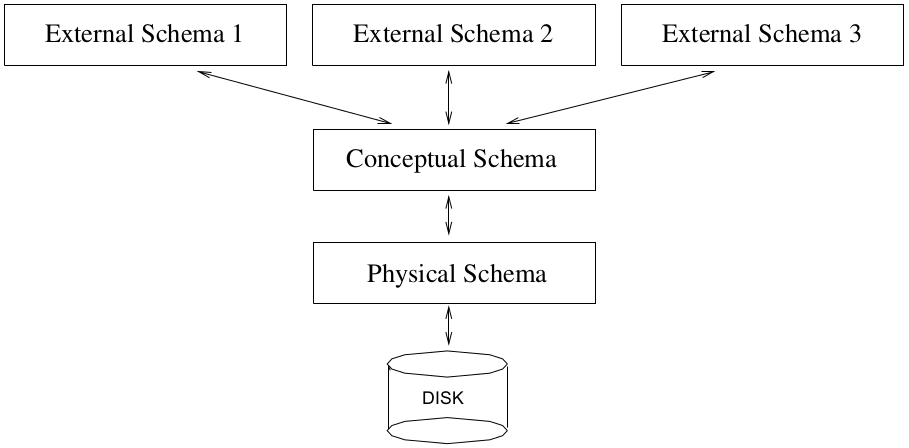
\includegraphics[width=0.65\columnwidth]{./img/dbms-abstraction-levels.png}
  \caption{Levels of abstraction in a DBMS (withdrawn from~\cite{ramakrishnan2003database})}%
\label{fig:dbms-abstraction-levels}
\end{figure}
%
\subsection{Transaction management}
\label{sec:trans-manag}
An important task of a \gls{dbms} is to schedule concurrent accesses to data in
a safe and seamless way to the user. Such accesses are named
\emph{transactions}, i.e., any one execution of a user program in a \gls{dbms},
corresponding to the basic unit of change as seen by the \gls{dbms}. Partial
transactions are not allowed, and the effect of a group of transactions is
equivalent to some serial execution of all transactions~\cite{ramakrishnan2003database}.

For the concurrent execution of transactions to take place, a \emph{locking
  protocol} is enforced by the \gls{dbms}, establishing a set of rules to be
followed by each transaction, using a \emph{lock} --- a mechanism to control
access to database objects.
Two kinds of locks are commonly supported by a DBMS: \emph{shared locks} on an
object can be held by two different transactions at the same time, but an
\emph{exclusive lock} on an object ensures that no other transactions hold any
lock on this object~\cite{ramakrishnan2003database}.

Transactions can be interrupted before running to completion for a variety of
reasons, e.g., a system crash. A DBMS must ensure that the changes made by such
incomplete transactions are removed from the database. To do so, the DBMS
maintains a log of all writes to the database, even before
the corresponding change is reflected in the database itself, enabling the
\gls{dbms} to detect and undo the changes if a system crash occurs. This property is called \gls{wal}. To ensure this property, the
DBMS must be able to selectively force a page in memory to disk~\cite{ramakrishnan2003database}.

The log is also used to ensure that the changes made by a successfully completed
transaction are not lost due to a system crash, as explained. Bringing
the database to a consistent state after a system crash can be a slow process,
since the DBMS must ensure that the effects of all transactions that completed
prior to the crash are restored, and that the effects of incomplete transactions
are undone. The time required to recover from a crash can be reduced by
periodically forcing some information to disk; this periodic operation is called a \emph{checkpoint}~\cite{ramakrishnan2003database}.

Summarizing, the main takeaways for \gls{dbms} support for concurrency control
and recovery are~\cite{ramakrishnan2003database}:
\begin{item-c}
\item \emph{Locking}:
every object that is read or written by a transaction is first locked in shared
or exclusive mode, respectively. Placing a lock on an object restricts its
availability to other transactions and thereby affects performance.
\item \emph{\gls{wal}}: for efficient log maintenance, the DBMS must be able to
  selectively force a collection of pages in main memory to disk. \gls{os}
  support for this operation is not always satisfactory.
\item \emph{Periodic checkpoint}:
  can reduce the time needed to recover from a crash. There is a trade-off
  between speed and system integrity, as checkpointing too often slows
  down normal execution. 
\end{item-c}
%
\subsection{Structure of a RDBMS}
\label{sec:structure-rdbms}

Fig.~\ref{fig:dbms-abstraction-levels} shows the structure (with some
simplification) of a typical \gls{dbms} based on the relational data model.
%
\begin{figure}[htb!]
\centering
    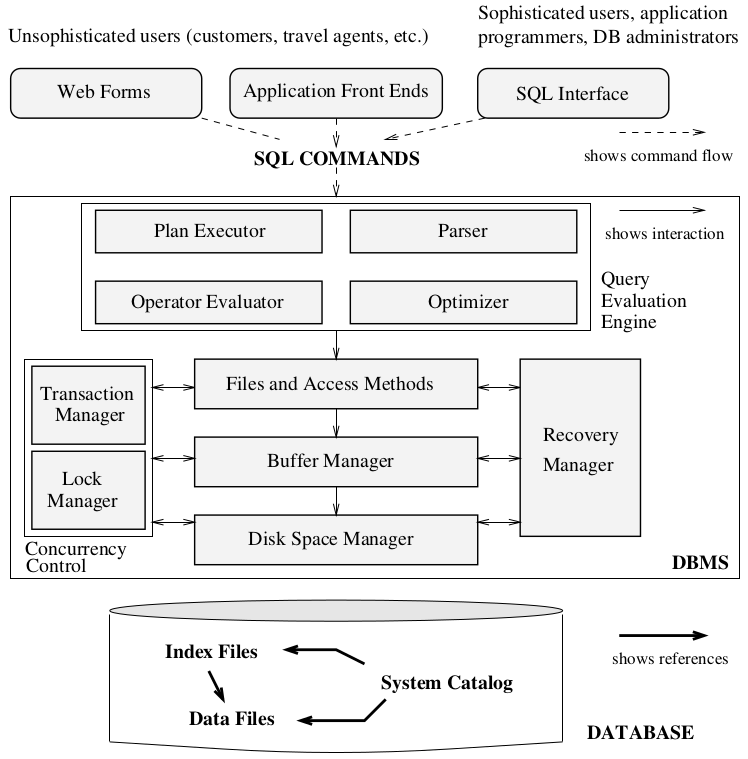
\includegraphics[width=0.75\columnwidth]{./img/dbms-struct.png}
  \caption{Architecure of a DBMS (withdrawn from~\cite{ramakrishnan2003database})}%
\label{fig:dbms-abstraction-levels}
\end{figure}
%

It is comprised of~\cite{ramakrishnan2003database}: 
\begin{item-c}
\item \emph{Interfaces}:
  The DBMS accepts \gls{sql} commands generated from a
  variety of user interfaces, produces query evaluation plans, executes these
  plans against the database, and returns the answers. SQL commands can also be
  embedded in host-language application programs, e.g., Java or C++ programs,
  but here one concentrates only on the core DBMS functionality.
\item \emph{\gls{dbms}}: contains:
  \begin{itemize}
  \item \emph{Query Evaluation Engine}:
    When a user issues a query, the parsed query is presented to a query
    optimizer, which uses information about how the data is stored to produce an
    efficient execution plan for evaluating the query. An execution plan is a
    blueprint for evaluating a query, and is usually represented as a tree of
    relational operators (with annotations that contain additional detailed
    information about which access methods to use, etc.).
  \item \emph{Concurrency control}:
  The \emph{Transaction Manager} ensures that transactions request and release
  locks according to a suitable locking protocol and schedules the execution
  transactions.
%
  The \emph{Lock Manager} keeps tracks of request for locks and grants locks on
  database objects when they become available.
 % 
  \item \emph{Recovery manager}:
    responsible for maintaining a log, and restoring the system to a consistent
    state after a crash.
  \item \emph{Disk access manager}:
    The \emph{file and access methods} layer includes a variety of software for
    supporting the concept of a file, which, in a DBMS, is a collection of pages
    or a collection of records. This layer typically supports a heap file, or
    file of unordered pages, as well as indexes.
    In addition to keeping track of the pages in a file, this layer organizes
    the information within a page.
%
    The \emph{Buffer manager} handles pages as a response to read requests.
%   
    The \emph{disk space manager} deals with management of space on
    disk, where the data is stored. Higher layers allocate, deallocate, read,
    and write pages through (routines provided by) this layer.
  \end{itemize}
\item \emph{Database}: contains the system catalog information consisting of the
  index files referencing the data files storing the actual data on physical
  memory.
\end{item-c}

\subsection{Database design overview}
\label{sec:datab-design-overv}
%
The database design process can be divided into six steps, namely~\cite{ramakrishnan2003database}:
\begin{enum-c}
\item \emph{Requirements Analysis}:
  the requirements for the database
  application are elicited and analyzed assessing what data is to be stored in
  the database, what applications must be built on top of it, and what operations are most frequent and subject to performance
  requirements.
Several methodologies have been proposed for organizing and presenting the
information gathered in this step, and some automated tools have been developed
to support this process.
\item \emph{Conceptual Database Design}:
the information gathered in the previous step is used to develop a high-level
description of the data to be stored in the database, along with the constraints that are known to hold over this data. This
step is often carried out using the \gls{er} model, or a similar high-level data model.
\item \emph{Logical Database Design}:
  A DBMS must be chosen to implement the database
design, and convert the conceptual database design -- \gls{er} schema --- into a database schema in the
data model of the chosen DBMS --- relational schema.
\item \emph{Schema Refinement}:
  Next, the collection of relations in the relation database schema are analyzed
  to identify potential problems, and to refine it. This is performed by
  normalizing relations, restructuring them to ensure some desirable
  properties.
\item \emph{Physical Database Design}:
  In this step, the typical expected workloads that the database must support
  are analyzed and further refine the database design to ensure that it meets
  desired performance criteria. This may simply involve building indexes on some tables and clustering some tables, or it may involve a substantial
  redesign of parts of the database schema obtained from the earlier design steps.
\item \emph{Security Design}:
  Lastly, the different user groups and different
roles played by various users are identified (e.g., the development team for a
product, the customer support representatives, the product manager).
For each role and user group, the permitted and forbidden parts of the database
are identified and the policies are enforced to ensure this. A DBMS provides
several mechanisms to assist in this step.
\end{enum-c}
%
\subsection{Entity-Relationship model}
\label{sec:entity-relat-model}
%
The \acrfull{er} data model enables the description of the data involved in a
real-world enterprise in terms of entities and their relationships and is widely
used to develop an initial database design. The \gls{er} model is most relevant
to the first three steps of the database
design~\cite{ramakrishnan2003database}~(see Section~\ref{sec:datab-design-overv}).
In this section are presented the
key concepts for the \gls{er} model as a database design modeling tool.
%

\subsubsection{Key concepts}
\label{sec:key-concepts}
It is important to understand some key concepts for the \gls{er} model, namely~\cite{ramakrishnan2003database}:
\begin{item-c}
\item \emph{Entity}: is an object in the real world that is distinguishable from
  other objects, e.g., the Pokemon toy, the toy department, the manager of the
  toy department, etc.
\item \emph{Entity set}: collection of entities. They do not need to be
  disjoint, i.e., entities can simultaneously belong to different entity
  sets. For example, one can define an entity set called \texttt{Employees} that
  contain both the toy and appliance department employee sets.
  An entity set is represented by a rectangle in the \gls{er} model.
\item \emph{Attributes}: an entity is described using a set of attributes. All
  entities in a given entity set have the same attributes. For example, the
  \texttt{Employees} entity set could use \texttt{name}, social security number
  (\texttt{ssn}) and parking lot (\texttt{lot}) as attributes.
  An attribute is represented by an oval in the \gls{er} model.
\item \emph{Domain}: for each attribute associated with a set, one must identify
  a domain of possible values. For example, the domain associated with the
  attribute \texttt{name} of \texttt{Employees} might be the set of 20-character
  strings.
  The domain information can be listed along the attribute name.
\item \emph{Key}: minimal set of attributes whose values uniquely identify an
  entity in the set. There could be more than one \emph{candidate} key: if so,
  one designate one of them as the \emph{primary} key.
  Each attribute in the primary key is underlined in the \gls{er} model. The
  \emph{foreign key} is(are) the
  attribute(s) which in a relationship one-to-many is(are) primary key(s) in the
  entity of the side \texttt{one} and integrates the set of attributes of the
  entity in the side \texttt{many} of that relationship
\item \emph{Relationship}: association between two or more entities.
  For example, one may have the relationship that Joe works in the pharmacy
  department.
  A relationship is represented by a straight line in the \gls{er} model and may
  also have \emph{descriptive attributes}.
\item \emph{Relationship set}: collection of similar relationships.
\item \emph{Key constraints}: restrictions over entities.
  For example, the restriction that each department has at most one manager, and
  is denoted by using an arrow from the entity to the relationship.
\item \emph{Participation constraints}: states the participation of an entity
  set in the relationship. It can be \emph{partial} or \emph{total}.
  For example, if every department is required to have a manager, the
  participation of the entity set \texttt{Departments} in the relationship set
  \texttt{Manages} is said to be \emph{total}.
\item \emph{Class hierarchies}: classification of entities in an entity set into
  subclasses, using the relationship \emph{is a}. For example, a \texttt{Car}
  \texttt{is a} \texttt{Vehicle} and a \texttt{Truck} \texttt{is a}
  \texttt{Vehicle} too. 
\item \emph{Aggregation}: indicates that a relationship set (identified through
  a dashed box) participates in another relationship set.
\end{item-c}

The \glspl{erd} use a graphical conventional to quickly and clearly depict the
entities involved and how they relate to each other. In a \gls{erd} entities are
represented by rectangles, attributes by ellipses, and the relationships as
lines between entities. In the rectangles and ellipses are placed the names of
the different entities and attributes. The relationships have cardinalities --- \texttt{1:1}
(one-to-one), \texttt{1:M} (one-to-many), and \texttt{M:N} (many-to-many) ---
and may be mandatory or optional --- e.g., a vehicle may not have any parking
space assigned, but to each parking space is assigned one, and one only,
vehicle.

Several notations can be used, namely, crow's foot, \gls{uml}, Chen, Barker,
etc~\cite{crowsfootNotation}.
In crow's foot notation:
\begin{item-c}
\item A multiplicity of one and a mandatory relationship is represented by a
  straight line perpendicular to the relationship line.
\item A multiplicity of many is represented by the three-pronged `crow-foot'
  symbol.
\item An optional relationship is represented by an empty circle.
\end{item-c}

Fig.~\ref{fig:erd-example} illustrates an example of an \acrfull{erd} using
crow's foot notation for an a company. There are three entity sets ---
\texttt{Customers}, \texttt{Orders}, and \texttt{Shipments}. Within each of
these are the attributes, with the primary key being underlined. Additionally it
also indicates the foreign key that resolves the \texttt{one-to-many}
relationship. Thus, a customer can place \texttt{0} or \texttt{many} orders, which, in
turn, can have \texttt{0} or \texttt{many} shipment methods.

%
\begin{figure}[htb!]
\centering
    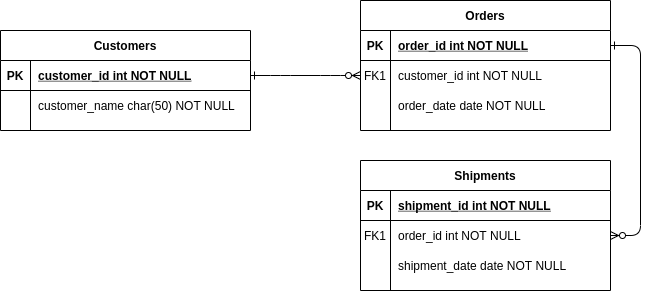
\includegraphics[width=0.8\columnwidth]{./img/erd-example.png}
  \caption{Example of an \gls{erd}}%
\label{fig:erd-example}
\end{figure}
%




\subsection{Choice of the RDBMS}
\label{sec:choice-rdbms}
In this section are presented the most relevant \glspl{rdbms}, focusing
specially on the open-source (and free) systems, namely \texttt{MySQL} and
\texttt{SQLite}.

The most relevant \glspl{rdbms} are~\cite{modernDBChoice}:
% src: https://www.xplenty.com/blog/which-database/
\begin{item-c}
\item \textbf{Oracle Database}: 
Oracle has provided high-quality database solutions since the 1970s. The most
recent version of Oracle Database was designed to integrate with cloud-based
systems, and it allows you to manage massive databases with billions of
records.
    \begin{itemize}
    \item \emph{Advantages}: the most advanced technology and a wide range of
    solutions.
    \item \emph{Disadvantages}: an expensive solution and system upgrades might be
    required ---  many businesses have to upgrade their hardware before using Oracle
    solutions.
    \item \emph{Best use case}: if you're a large organization that needs to manage
    a massive amount of data, Oracle could be the ideal choice.
  \end{itemize}
\item \textbf{Microsoft SQL Server}: it is a database engine that is compatible
  with, both, on-site and cloud-based servers, and supports Windows and Linux
  OSes.
    \begin{itemize}
    \item \emph{Advantages}: it is mobile: this database engine allows you to
      access dashboard graphics and visuals via mobile devices. It integrates
      with Microsoft products.  It is fast and stable.
    \item \emph{Disadvantages}: an expensive solution and requires a lot of
      \gls{hw} resources.
    \item \emph{Best use case}: if you're an enterprise-level corporation that
      relies heavily on Microsoft products, the speed, agility, and reliability
      of Microsoft SQL Server could be an excellent choice.
  \end{itemize}
\item \textbf{MySQL}: MySQL is a free, open-source RDBMS solution that Oracle
  owns and manages. Even though it's freeware, MySQL benefits from frequent
  security and features updates. Large enterprises can upgrade to paid versions of MySQL to benefit from additional features and user support.
    \begin{itemize}
    \item \emph{Advantages}: it is open-source, free of charge (freeware) and
      highly compatible with many other database systems.
    \item \emph{Disadvantages}: lacking features common to other \glspl{rdbms}:
      because MySQL prioritizes speed and agility over features, some of the
      standard features found in other solutions may be missing, e.g., the
      ability to create incremental backups. Challenges getting quality support:
      The free version of MySQL does not come with on-demand support. However,
      MySQL does have an active volunteer community, useful forums, and a lot of
      documentation.
    \item \emph{Best use case}: MySQL is a particularly valuable RDBMS solution
      for businesses that need a solution with enterprise-level capabilities,
      but are operating under strict budget constraints. It is an extremely
      powerful and reliable modern RDBMS with a free tier.
  \end{itemize}
\item \textbf{SQLite}:
\end{item-c}

\subsection{SQL}
\label{sec:sql}
Ideally, a database language allows the creation of a database and table
structures, the execution of basic data management tasks (add, delete, and
modify), and the execution of complex queries designed to transform the raw data
into useful information. Moreover, it must provide a clear and easy suntax, it
must be portable and conform to some basic standard. \gls{sql} complies well to
these requirements~\cite{coronel2016database}.

\gls{sql} functions fit into two broad categories~\cite{coronel2016database}:
\begin{enum-c}
\item It is a \emph{\gls{ddl}}: SQL includes commands to create database objects
  such as tables, indexes, and views, as well as commands to define access
  rights to those database objects (see Fig.~\ref{fig:sql-dll}).
\item It is a \emph{\gls{dml}}: SQL includes commands to insert, update, delete,
  and retrieve data within the database tables (see Fig.~\ref{fig:sql-dml}).
\end{enum-c}
%
\begin{figure}[htb!]
\centering
    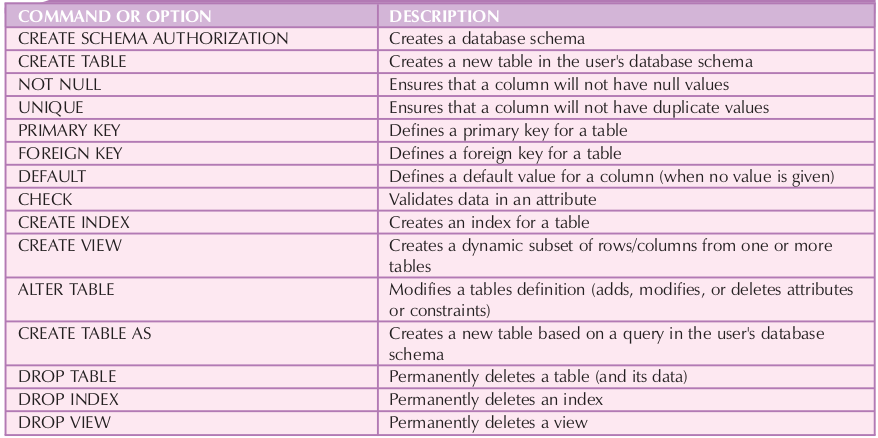
\includegraphics[width=0.9\columnwidth]{./img/sql-dll.png}
  \caption{SQL data definition commands --- withdrawn from~\cite{coronel2016database}}%
  \label{fig:sql-dll}
\end{figure}
%
\begin{figure}[htb!]
  \centering
  % 
  \begin{subfigure}[t]{.9\textwidth}
  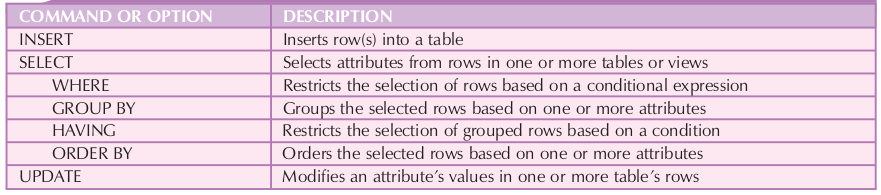
\includegraphics[width=\textwidth]{img/sql-dml-1.png}%
  %\caption{main}%
  %\label{fig:state-mach-local-superv-main}
\end{subfigure}
%
%\vspace{-0.1\textwidth}
%
  \begin{subfigure}{.9\textwidth}
  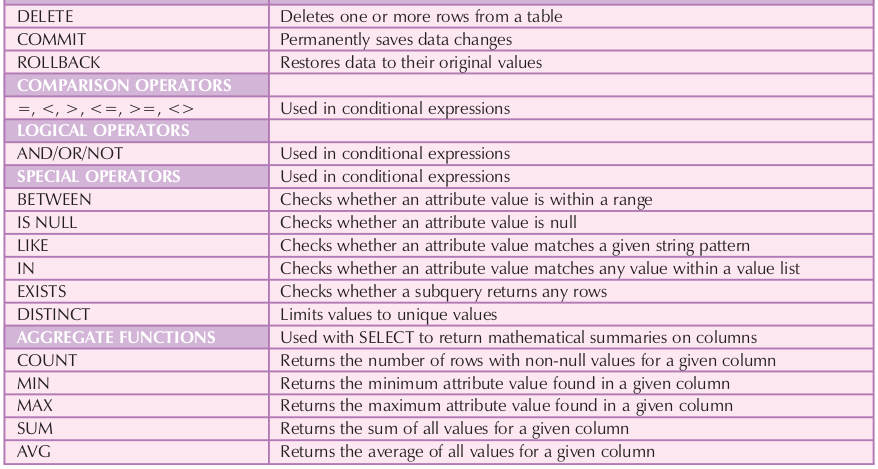
\includegraphics[width=\textwidth]{img/sql-dml-2.png}%
  %\caption{Mode Manager}%
  %\label{fig:state-mach-local-superv-mode}
\end{subfigure}
  % 
  \caption{SQL data manipulation commands --- withdrawn from~\cite{coronel2016database}}%
  \label{fig:sql-dml}
\end{figure}
%


\subsection{SQL C++ interface}
\label{sec:sql-c++-interface}





%% Local Variables:
%% mode: latex
%% TeX-master: "../../../dissertation"
%% End:

% cli-serv
%
\section{Motion detection}
\label{sec:motion-detection}
The \texttt{\gls{mdo-l}} needs to be capable of detecting a user, in order to switch between \texttt{normal mode} to \texttt{interaction mode}.
In order to do such thing, it is mandatory to have a system that detects the motion of a user that approaches to the local system \texttt{\gls{mdo-l}}.

\subsection{Different types of detection}
There are several ways to do motion detection, through different sensors, such as~\cite{sensors-list}:
%
\begin{itemize}
\item \emph{\gls{pir}}: A passive infrared sensor detects body heat (infrared energy) by looking for changes in temperatures. 
This is the most-widely-used motion sensor in home security systems~\cite{sensors-list}.

Once the PIR motion sensor warms up, it can detect heat and movement in the surrounding areas, creating a protective "grid".
If a moving object blocks too many grid zones and the infrared energy levels change rapidly, the infrared sensor triggers an alarm~\cite{sensors-list}.
%
\item \emph{\gls{mw}}: This type of sensor sends out microwave pulses and measures the reflections off of moving objects.
They cover a larger area than infrared sensors but are more expensive and vulnerable to electrical interference~\cite{sensors-list}.
%
\item \emph{Dual technology motion sensors}: Some motion sensors can combine multiple detection methods in an attempt to reduce false alarms.
For example, it's not uncommon for a dual technology sensor to combine a \gls{pir} sensor with a \gls{mw} sensor~\cite{sensors-list}.
%
\item Less common types of motion detectors:
	\begin{item-c}
	\item \emph{Area reflective sensors}: This kind of sensors emit infrared rays from an LED and use the reflection of those rays to measure the distance to the person or object, allowing for detection when the subject moves within the designated area~\cite{sensors-list}.
	%
	\item \emph{Ultrasonic motion sensors}: This sensors measure the reflections off of moving objects via pulses of ultrasonic waves~\cite{sensors-list}.
	%	
	\item \emph{Vibration motion sensors}: This type of sensors detect small vibrations that people cause when they move through a room~\cite{sensors-list}.
	\end{item-c}
	%
\item Specialized motion sensors:
	\begin{item-c}
	\item \emph{Contact sensors}: Contact sensors use a magnet to spot movement on a door or window. When the sensor and corresponding magnet move apart as a door or window opens, the sensor triggers~\cite{sensors-list}.
	%
	\item \emph{Pet-immune motion sensors}: Most passive infrared sensors can ignore animals up to a certain weight. A dual technology motion sensor is more pet resistant to false alarms because it requires two sensors to be triggered a certain way~\cite{sensors-list}. 
	%	
	\end{item-c}
\end{itemize}

\subsection{Trade-off between sensors}
As it can be seen previously, there are several types of sensors that can be used. However, it is mandatory to make a trade-off between each type in order to choose the better case, according several factors such as price, range, applicability, conditions of use and others.

For this specific case, it is necessary a set of sensors with a low range detection (more or less than 1,5 meters), a good reflection and low consumption. Thus, the type of sensors that match all these criteria are ultrasonic sensors.
The reasons to discard the others sensors are simple:

Firstly, the \gls{pir} sensor actuates with changes in radiation, which means that some other case can occur where is not a human approaching the \gls{mdo-l} like, for example, an animal.

In second place, the Infrared Reflective sensors have too specific characteristics of behavior. 
For example, there are some surfaces that do not reflect quite good the \gls{ir} radiation, which could easily result on a bad behavior for two different users.

Lastly, the contact sensors are out of question for obvious reasons: there is no need to have a contact between the \gls{mdo-l} and an user.

Concluding, the best option is to use a set of ultrasonic sensors, in order to avoid some specific situations and make the user detection as better as possible.

\subsection{Ultrasonic sensor}
Ultrasonic sensors work by sending out a sound wave at a frequency above the range of human hearing.
Ultrasonic waves are sound waves emitted at a frequency higher than can be detected by human hearing — typically above 20 kHz~\cite{ultrasonic-sensor-img}.

As it can be seen in Fig.~\ref{fig:ultrasonic-sensor}, many ultrasonic sensors use a single transducer to send a pulse and to receive the echo, others use one transducer to send the pulse and another to receive it.  
The sensor determines the distance to a target by measuring time lapses between the sending and receiving of the ultrasonic pulse~\cite{ultrasonic-sensor}.

\begin{figure}[!hbt]
\centering
    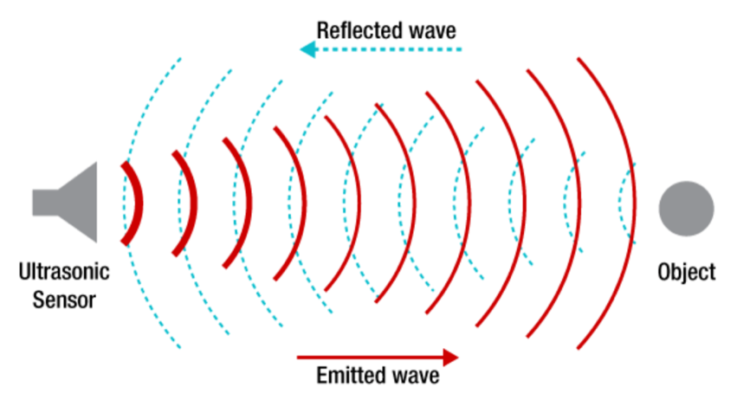
\includegraphics[width=0.6\textwidth]{./img/ultrasonic-sensor.png}
  \caption{Example of the behaviour of an ultrasonic sensor(withdrawn from~\cite{ultrasonic-sensor-img})}%
\label{fig:ultrasonic-sensor}
\end{figure}

%%% Local Variables:
%%% mode: latex
%%% TeX-master: "../../../dissertation"
%%% End:

% cli-serv
%
\section{Camera recording and codecs}
\label{sec:camera-record-codecs}

In this project's local system (\gls{mdo-l}), the \texttt{Interaction Mode} is composed by an interaction made through video between the machine and the user.
To make possible that interaction through video, it is necessary to know how to record and show the frames captured by the camera using the Raspberry Pi. 

The process of recording is just simply capture several frames in a specific period and then when all frames are joined together it creates a video.
The more frames are captured per second, the more fluid the video becomes, that's why it is normal to talk about \gls{fps} when talking about video recording or playing.

\subsection{Camera recording}
\label{sub-sec:camera-record}
It is possible to capture video from the raspberry using its camera module (V2) with the help of the \texttt{OpenCV} library.
With a simple code in C++, it is possible to capture frames and show them in loop, in order to always refresh what the camera is recording.
Listing \ref{lst:camera-example} implements how to show what is being captured by the camera. Basically it is created a variable \texttt{frame} to read the frames of the camera and the \texttt{cap} refers to the camera (which in this case has 0 that represents the camera ID).
Then, basically it is just needed to verify if the camera is opened and if so read the frame from the camera and show it. This last two steps are executed in a infinite loop until a key is pressed to stop the execution. 
%
\lstinputlisting[language=C++,firstline=1,
caption={Example of camera frames acquisition (withdrawn from \cite{camera-example})},
label=lst:camera-example,
style=custom-cpp]{./listing/camera-example.cpp}

\subsection{Video files encoding (codecs) and formats}
\label{sub-sec:codecs-and-formats}
Video encoding formats, also called video file formats, are methods of optimizing digital video files for different platforms, programs, and devices.
There are many different kinds of video encoding formats, but each is composed of two main parts: a \texttt{codec} and a \texttt{container}~\cite{video-encoding}. But firstly, it is necessary to know how video encoding works.

Video encoding is the process of turning uncompressed video input into a form that can be stored and played by a variety of devices and thisi envolves two main processes: \texttt{compression} and \texttt{transcoding}~\cite{video-encoding}.
%
\begin{item-c}
\item \emph{Compression}: decreases the size of a video file so that it is more manageable. Without proper compression, most files would be far too large to upload easily, load quickly, or play smoothly on users' devices.
\item \emph{Transcoding}: refers to the total audio and video conversion process from one video format to another. It ensures that a video file is compatible with the video player and/or platform it is using. Without transcoding, users would not be able to watch the video file at all.
\end{item-c}

On-demand streaming video is encoded so that it can be sent over the Internet and played on a variety of user devices. During live streaming, the video stream is segmented, compressed, and encoded in real time~\cite{video-encoding}.

\subsubsection{What is a codec?}
A codec (coder/decoder) is a method for compressing and decompressing data so that it can be easily transported and received by different applications. Separate codecs are used to compress audio and video files, but they generally work in the same way~\cite{video-encoding}.
Codecs encode files using either lossy compression or lossless compression. Lossy compression simplifies the data in a video file and only keeps the essential parts. This is why a video using lossy compression may look pixelated or "fuzzy"~\cite{video-encoding}. 

\subsubsection{What is a container?}
A container combines an encoded audio stream (audio codec), encoded video stream (video codec), and metadata in a single video file. The metadata tells the video player how to coordinate different audio and video codecs and may also provide additional elements, such as subtitles or alternate audio streams~\cite{video-encoding}.
Each container supports a different range of video codecs. Some containers only work with a single type of codec and video player, which drastically limits playback options. Other containers are compatible with many types of video codecs and players~\cite{video-encoding}.

\subsubsection{Most common types of video formats}
There are many types of video encoding formats and they are not compatible with the same platforms, browsers and devices.
These are the most common video formats~\cite{video-encoding}:
\begin{item-c}
\item \emph{MP4}: is a video file format created by the Motion Picture Expert Group. It compresses audio and video separately, which allows MP4 files to retain relatively high video quality after compression. Most browsers and iOS/Android devices are compatible with MP4 files.
%
\item \emph{MOV}: is a video file format created by Apple. Although it can run on both Mac OS and Windows OS, it is only compatible with QuickTime video players. It preserves video quality, but does not offer as much file compression as other common video formats, such as MP4.
%
\item \emph{AVI}: is a video file format created by Microsoft. It is one of the oldest video file container specifications. AVI works with a number of different codecs, which can affect how well it is supported by different operating systems and browsers. It prioritizes video quality over compression, meaning that video files are larger and better quality overall.
%
\item \emph{FLV}: is a video file format created by Adobe Flash. A clear advantage of FLV is its ability to compress video files without severe loss of video quality. However, it is far less compatible across devices and OSes than other file formats: Though it is supported by most browsers and Android devices, it cannot be used to play any video files on iOS devices like iPhones or iPads. Browsers have dropped support for Adobe Flash because it is considered to be insecure, and Adobe no longer supports Flash.
%
\item \emph{WebM}: is a video file format developed by Google. It is a subset of the open-standard Matroska Video Container (MKV) format, which is highly adaptive to most video and audio codecs and compatible with a wide range of platforms and devices. WebM is a web-friendly, open-source alternative to MP4 that maintains high video quality after compression.
\end{item-c}

\subsection{Video players for Raspberry Pi}
\label{sub-sec:video-player}
It is necessary to have a video player in the Raspberry Pi, in order to play the video that are encoded.
The more extendable the player is, the more easier and practical it is to use.
There are two main video players that can be used on Raspberry~\cite{video-player-rasp}:
%
\begin{item-c}
\item \emph{VLC}: is one of the best video players that one can install on the Raspberry Pi. It will play almost any video and audio format that one throws at it. This means that it's not needed to spend time finding particular codecs to get videos or music playing on Raspberry Pi.
\item \emph{OMXPlayer}: is a video player for the Raspberry Pi that can run completely from the terminal. This video player has been heavily optimized for the Raspberry Pi's hardware and was designed originally as a testbed for the Kodi media player. While OMXPlayer does not have as a wide range of support as VLC, it still has its uses for those who don't want a full-blown video player.
\end{item-c}

In conclusion, for this project the best video player that can be used is the \texttt{OMXPlayer} for its capability of running completely in the terminal, which can be a very useful feature in several cases such as testing through the \texttt{Admin Remote Client} the operation of the \gls{mdo-l}.

\subsection{Playing video in C++}
\label{sub-sec:play-video-cpp}
Although there's already a solution to play videos through terminal, it is also necessary to play videos in the \gls{ui} and for that case it is mandatory to have a library that can do video playback.

One library that is very useful to do playback is the \texttt{OpenCV} library, having the advantage that this is already used in other subsystems of the project.
This library has also the advantage of working compatibly with the chosen \texttt{ui} (explained later on section \ref{sec:ui-framework}). 

\subsubsection{Example of video playback}
Here's an example on how to play a video using this library in C++:

Firstly, the definition of the \texttt{Player()} class that handles the video playback.
Listing \ref{lst:video-play-cpp-class} shows the \texttt{Player()} class that needs the \texttt{frame} to do the acquisition of the frames of the video, the \texttt{frameRate} to know the video frame rate and the \texttt{img} that is used to show the frame.
%
\lstinputlisting[language=C++,firstline=1,
caption={Example of video playback in OpenCV uisng C++ - Player class (withdrawn from \cite{video-play-cpp})},
label=lst:video-play-cpp-class,
style=custom-cpp]{./listing/video-play-class.cpp}
%
Then, listing \ref{lst:video-play-cpp} shows the implementation of the main member functions.
Firstly, the \texttt{loadVideo} function loads the video and reads the framerate of the video.
Then, the \texttt{run} function reads the frame from the video, attributes it to the \texttt{img} to be then showed on the widget and finally waits the specific time to show the next frame in order to respect the video's frame rate, all this execution occurs while the video doesn't stop.
Lastly, the \texttt{updatePlayerUI} puts the image on the widget using the functions that \texttt{Qt} already gives.
%
\lstinputlisting[language=C++,firstline=1,
caption={Example of video playback in OpenCV uisng C++ - Player class implementation(withdrawn from \cite{video-play-cpp})},
label=lst:video-play-cpp,
style=custom-cpp]{./listing/video-play.cpp}
%%% Local Variables:
%%% mode: latex
%%% TeX-master: "../../../dissertation"
%%% End:

% cli-serv
%
\section{Image filtering}
\label{sec:image-filtering}
aaaaaaaa


%%% Local Variables:
%%% mode: latex
%%% TeX-master: "../../../dissertation"
%%% End:

% cli-serv
%
\section{GIF generation}
\label{sec:gif-generation}
aaaaaaaa


%%% Local Variables:
%%% mode: latex
%%% TeX-master: "../../../dissertation"
%%% End:

% cli-serv
\section{Social media sharing APIs}
\label{sec:social-media-sharing}
Social media platforms are great contact points to target customers and to
increase brand awareness, which is highly desirable for digital marketing. These
platforms provide a set of functionalities to external agents interact with them
in a programmatic way, enabling automation of tasks like content sharing,
scheduling, search, etc.
These functionalities are exposed by \glspl{api}, providing a custom and
well-defined interface that can be explored by developers to build custom
applications that leverages on them.

There are several social media platforms, but here one focuses on the most
popular ones, namely~\cite{rakutenTop10SMApis, ayrshareTop10SMApis}:
\begin{enum-c}
\item \emph{Facebook}:
  Facebook is a social networking platform that allows users to communicate
  using messages, photos, comments, videos, news, and other interactive content.
  \begin{itemize}
  \item \emph{API features}:
    Facebook provides various \glspl{api} and \glspl{sdk} that allow developers to access its
    data and extend the capabilities of their applications. The Facebook Graph
    API is an \gls{http}--based API that provides the main way of accessing the
    platform's data. With the API, one can query data, post images, access
    pages, create new stories, and carry out other tasks. Furthermore, the
    Facebook Marketing API allows one to create applications for automatically
    marketing one's products and services on the platform.
  \item \emph{Popularity}:
    At the end of 2018, Facebook was boasting of more than 2.2
    billion monthly active users, making it the most popular social media
    platform in the world.
  \item \emph{Price}:
    The Facebook APIs --- Graph API --- are provided for free.
  \item \emph{Ease of use}:
    Apart from its detailed documentation, Facebook has an active
developer community with members who are always willing to assist each other
make the most of them. The API is large, documentation decent and leans towards
PHP, and requires the developer to create a video or screencast to be approved.
\item \emph{Registration process}: the developer needs to register its app, and if for
  commercial purposes, register its business. This includes verifying his/her legal entity and address.
  \end{itemize}
%
\item \emph{Instagram}:
Instagram is a Facebook-owned social networking platform that lets users share
photos and videos.
%
\begin{itemize}
\item \emph{API features}:
  Facebook offers many APIs to allow developers to create tools that enhance
  users' experience on the Instagram platform. With the APIs, one can enable
  users to share their favorite stories and daily highlights from one's
  application to Instagram. Furthermore, there is the Instagram Graph API that
  allows developers to access the data of businesses operating Instagram
  accounts. With the Graph API, one can conveniently manage and publish media
  objects, discover other businesses, track mentions, analyze valuable metrics,
  moderate comments, and search hashtags.
\item \emph{Popularity}:
  At the end of 2018, Instagram had more than 1 billion monthly active users.
\item \emph{Price}:
  The APIs are offered for free.
\item \emph{Ease of use}:
  The Instagram APIs are easy to use. Facebook has done good
  work in providing detailed documentation to assist developers in easily
  implementing the APIs into their applications.
\item \emph{Registration process}: subject to the same terms of Facebook
  registration process. Additionally, the API allows the developer to pull data, but it can
  not post via the API unless he's/she's a `Partner'. The partner
 program started in 2018 and isn't open to new partners unless Instagram asks
 one to join.  
\end{itemize}
%
\item \emph{Twitter}:
Twitter is a popular social media service that allows users to find the latest
world events and interact with other users using various types of messaging
content (called tweets). Twitter can be accessed via its website interface,
applications installed on mobile devices, or a short message service (SMS).
\begin{itemize}
\item \emph{API features}:
  Twitter provides various API endpoints for completing various tasks. For example, one can use the Search API to retrieve historical tweets, the Account Activity API to access account activities, the Direct Message API to send direct messages, Ads API to create advertisement campaigns, and Embed API to insert tweets on one's web application.
\item \emph{Popularity}:
Twitter is a very popular social media networking service that can assist in enhancing the engagement of one's application. At the end of 2018, it had more than 335 million monthly active users.
\item \emph{Price}:
Twitter provides its APIs for free. However, if one want a high level of access and reliability, one’ll need to contact them for paid API versions.
\item \emph{Ease of use}:
Ease of use: The Twitter APIs are very easy to use. Twitter provides
comprehensive documentation to assist one in flawlessly integrating any of its
APIs into one's specific use case. Some API wrappers are also available in
several programming languages. The new Twitter developer site no longer allows
localhost in their approved callback URLs, so one’ll need to use \texttt{ngrok} or an equivalent tunnel to test locally.
\item \emph{Registration process}: it requires the application to be registered as a
  new project (using Twitter's Developer interface) and the developer can get a
  permanent access token. Much easier than for the other two platforms.
\end{itemize}
\end{enum-c}

The social media \glspl{api} are specific to each platform. Thus, developing a
custom interface for each of these platforms is a very time consuming
task. Instead, one will focus only on one social media platform, and its
associated \gls{api}. The chosen platform is \textbf{Twitter} as it's the less
extent and more easy to implement and its registration process is the least cumbersome.

\subsection{Twitter API}
\label{sec:twitter-api}
The Twitter API can be used to programmatically retrieve and analyze Twitter
data, as well as build for the conversation on Twitter. Over the years, the
Twitter API has grown by adding more levels of access for developers and
academic researchers to be able to scale their access to enhance and research
the public conversation. Recently, the Twitter API v2 has been released,
including a modern foundation, new and advanced features, and quick on-boarding
to Essential access~\cite{twitterAbout}.

To get access to the Twitter \gls{api}, the developer needs to~\cite{twitterAPIGettingStarted}:
\begin{enum-c}
\item
  \emph{Sign up for a developer account}: After signing-up, one will create a
  Project and an associated developer App during the on-boarding process, which
  will provide a set of credentials that will be used to authenticate all
  requests to the API.
\item
  \emph{Save the Application's keys and tokens and keep them secure}:
After completing step 1, one will be able to find or generate the following
credentials within one's developer App:
\begin{itemize}
\item 
    \emph{API Key and Secret}: Essentially the username and password for one's App. One
    will use these to authenticate requests that require OAuth 1.0a User
    Context, or to generate other tokens such as user Access Tokens or an
    app-only Bearer Token.
  \item 
    \emph{A set of user Access Tokens}: In general, Access Tokens represent the user
    that one are making the request on behalf of. The ones that one can generate
    via the developer portal represent the user that owns the App. One will use
    these to authenticate requests that require OAuth 1.0a User Context. If one
    would like to make requests on behalf of another user, one will need to use
    the 3-legged OAuth flow for them to be authorized. 
  \item 
    \emph{Bearer Token}: One will use this token when making a request to an endpoint that requires OAuth 2.0 Bearer Token.
\end{itemize}

\item
  \emph{Make the first request}: after completing the first two steps, one can
  use the \gls{api} to interact with the Twitter platform.
\item
  \emph{Apply for additional access}:
  With Essential access, one is only able to make requests to the Twitter API v2
  endpoints, and not the v1.1 or enterprise endpoints.  One is limited to 500K Tweets/month, and unable to take advantage of certain developer portal functionality such as teams and access to additional App environments. 

If one wants to access the standard v1.1, premium v1.1, or enterprise endpoints,
or if one wants to take advantage of an increased Tweet cap and developer portal
functionality, one needs to apply for Elevated or Academic Research access. 
\end{enum-c}

It is important to note that the Twitter \gls{api} is a \gls{rest}
(a.k.a. \gls{rest}ful) \gls{api}, which means that when a client request is made
through it, it transfers a representation of the state of the resource to the
requester or endpoint. This information, or representation, is delivered in one
of several formats via \gls{http}: \gls{json}, \gls{html}, XLT (Excel
Templates), Python, PHP, or plain text. The Twitter API uses \gls{json} --- the most
generally popular file format to use, because, despite its name, it’s language-agnostic, as well
as readable by both humans and machines~\cite{whatsRestApi}.

\gls{rest} is a set of architectural constraints, not a protocol or a
standard. API developers can implement \gls{rest} in a variety of ways, making
REST APIs faster and more lightweight, with increased scalability --- perfect
for \gls{iot} applications and mobile app development~\cite{whatsRestApi}.

Another important note about RESTful APIs: headers and parameters are also important in the HTTP methods of a RESTful API HTTP request, as they contain important identifier information as to the request's metadata, authorization, uniform resource identifier (URI), caching, cookies, and more. There are request headers and response headers, each with their own HTTP connection information and status codes~\cite{whatsRestApi}.

For an API to be considered RESTful, it has to conform to the following
criteria~\cite{whatsRestApi}:
\begin{item-c}
\item A client-server architecture made up of clients, servers, and resources,
  with requests managed through HTTP.
\item Stateless client-server communication, meaning no client information is
  stored between get requests and each request is separate and unconnected.
\item Cacheable data that streamlines client-server interactions.
\item A uniform interface between components so that information is transferred
  in a standard form. This requires that:
  \begin{itemize}
    \item resources requested are identifiable and separate from the
      representations sent to the client.
    \item resources can be manipulated by the client via the representation they
      receive because the representation contains enough information to do so.
    \item self-descriptive messages returned to the client have enough
      information to describe how the client should process it.
    \item hypertext/hypermedia is available, meaning that after accessing a
      resource the client should be able to use hyperlinks to find all other
      currently available actions they can take.
  \end{itemize}
\item A layered system that organizes each type of server (those responsible for
  security, load-balancing, etc.) involved the retrieval of requested
  information into hierarchies, invisible to the client.
\item Code-on-demand (optional): the ability to send executable code from the
  server to the client when requested, extending client functionality.
\end{item-c}

To interact with the \texttt{Twitter} platform, one can make a request and
retrieve its response by following these steps~\cite{twitterAPIMakeFirstRequest}:
\begin{enum-c}
\item \emph{Select the end-point}: several actions can be performed on the
  Twitter website on mobile application, varying its interface.
\item \emph{Select a tool to make the request}: one can use command line tools,
  driver programs or libraries in several programming languages, or tools like
  Postman and Imsonia --- visual tools to make requests to \gls{rest} endpoints.
%
  For example, here is a \texttt{cURL} example for the user lookup endpoint.
  To use this request the \texttt{BEARER\_TOKEN} and \texttt{USERNAME} with
  Bearer Token and Twitter handle of the developer, and execute it in the
  command line.
  \begin{quote}
      \onehalfspacing
\begin{verbatim}
curl "https://api.twitter.com/2/users/by/username/$USERNAME" -H 
"Authorization: Bearer $BEARER_TOKEN"
\end{verbatim}
  \end{quote}
    \vspace{-2mm}
  %
\item \emph{Review the response}:
  Once a successful request has been made, a payload will be received with
  metadata related to the request.
  \begin{itemize}
  \item 
  If you used an endpoint that utilizes a GET HTTP method, you will receive
  metadata related to the resource (Tweet, user, List, Space, etc) that you made
  the request to in JSON format. Review the different fields that returned and
  see if you can map the information that you requested to the content on
  Twitter.
\item 
If you used an endpoint that utilizes a POST, PUT, or DELETE HTTP method, you performed an action on Twitter. Go to Twitter.com or the mobile app and see if you can track down that action. 
  \end{itemize}
%
\item \emph{Adjust the request using parameters}:
  Each endpoint has a different set of parameters that can be used to alter the
  request. For example, additional metadata fields can be requested when using
  GET endpoints with the fields and expansions parameters.
\end{enum-c}

\subsubsection{Manage Tweets example}
\label{sec:manage-tweets-exampl}
Creating and deleting Tweets using the Twitter API is essential for engaging
with the public conversation. There are two available methods to manage Tweets~\cite{twitterManageTweetIntro}:
\begin{enum-c}
\item \emph{\texttt{POST}}: it allows one to post polls, quote Tweets, Tweet
  with reply settings, Tweet with geo, Tweet with media and tag users, and Tweet to Super Followers, in addition to other
  features. It can be further customized using parameters.
There is a user rate limit of 200 requests per 15 minutes for the POST
method.
\item \emph{\texttt{DELETE}}: allows to delete a specific Tweet.
It has a rate limit of 50 requests per 15 minutes.
\end{enum-c}

Since one is making requests on behalf of a user with all manage Tweets
endpoints, one must authenticate with OAuth 1.0a User Context and use the Access
Tokens associated with a user that has authorized one's App. The Access Tokens
can be generated using the 3-legged OAuth flow.

As an example let's focus on the \textbf{post tweet} feature. For this purpose, one needs
to~\cite{twitterManageTweetQuickStart}:
\begin{enum-c}
\item \emph{Select a tool or library to make the request}:
  Postman, Imsonia,
  driver programs or libraries in several programming languages. In this case,
  one will consider \texttt{cURL} and the command line.
\item \emph{Authenticate the request}:
  To make a successful request to this endpoint, one will need to use OAuth 1.0a
  User Context. To do this, the following keys and tokens must be added to the
  shell environment by exporting the following variables:
  \begin{itemize}
    \item \texttt{consumer\_key} with your API Key
    \item \texttt{consumer\_secret} with your API Key Secret
    \item \texttt{access\_token} with your Access Token
    \item \texttt{token\_secret} with your Access Token Secret
    \end{itemize}
  \item \emph{Configure the request with parameters}: one can inspect the
    \texttt{POST /2/tweets} API call to understand its usage and
    configuration~\cite{twitterAPIRefPostTweet}. Some relevant parameters are:
    \texttt{text} --- a string containing the text of the Tweet; \texttt{media}
    --- a \gls{json} object containing the media information being attached to
    the tweet. Here, one will use just the first.
  \item \emph{Make the request}: using \texttt{cURL} one has:
    \begin{quote}
      \onehalfspacing
        \begin{verbatim}
        curl -X POST https://api.twitter.com/2/tweets -H 
        "Authorization: OAuth \$OAUTH_SIGNATURE" -H 
        "Content-type: application/json" -d '{"text": "Hello World!"}'
        \end{verbatim}
    \end{quote}
    \vspace{-7mm}
%
  \item \emph{Analyze the response}: an example response can be the following
    \gls{json} object,
    containing the \texttt{id} and the \texttt{text} of the newly created tweet.
    \begin{quote}
      \onehalfspacing
        \begin{verbatim}
        {
            "data": {
                "id": "1445880548472328192",
                "text": "Hello world!"
            }
        }
        \end{verbatim}
    \end{quote}
    \vspace{-7mm}
  \end{enum-c}

  

%%% Local Variables:
%%% mode: latex
%%% TeX-master: "../../../dissertation"
%%% End:

\subsubsection{C++ libraries and APIs}
\label{sec:c++-libraries-apis}
The Twitter \gls{api} is a \gls{rest}ful \gls{api}, which, in practical terms,
means that \gls{http} headers can be used to send (\texttt{POST}) and retrieve
data (\texttt{GET}) from the Twitter platform.

Thus, one only requires an wrapper around these \gls{http} `methods' to
interface Twitter. One such tool, as aforementioned, it's \texttt{cURL} ---
client \gls{url}, a
command-line utility for transferring data with \glspl{url}~\cite{curl}. It is a free,
open-source tool developed in C++, first released in 1997. cURL offers
`\texttt{libcurl}', a library, and `\texttt{curl}', a command-line tool, and is
often used to retrieve data from Twitter~\cite{twitterCreatingLibsC}.

Several C++ \glspl{api} are available for Twitter, although not officially
recommended by Twitter:
\begin{enum-c}
\item \texttt{kQOAuth} by Johan Paul --- a Qt based OAuth Library;
\item \texttt{libOAuth} by Robin Gareus --- a collection of POSIX-C functions implementing OAuth;
\item \texttt{QTweetLib} by Toni Jovanoski --- a Qt based Twitter API library;
\item \texttt{Twitcurl} by Mahesh --- a Twitter API library;
\end{enum-c}

There are two \texttt{Qt} based libraries, thus making it
highly-dependent on the \texttt{Qt} platform, a collection of POSIX-C functions
implementing only the authentication mechanism, and a pure C++ \gls{api} library
for Twitter. Hence, from the above two options arise for building the
\texttt{Local System}'s interface for Twitter:
\begin{enum-c}
\item \emph{\texttt{libcurl}}: a free and easy-to-use client-side URL transfer library
  with a C \gls{api}~\cite{libcurl}. One could then write a C++ wrapper around it to follow
  \gls{oop} paradigm or use the one of the recommended wrappers ---
  \texttt{curlpp}, \texttt{curlcpp}, or \texttt{C++ Requests} --- and then write
  a wrapper to handle Twitter requests~\cite{libcurlBindings};
\item \emph{\texttt{Twitcurl}}~\cite{twitcurlGithub}: use a pure C++ \gls{api} to interface \texttt{Twitter},
  providing a straightforward mechanism to handle requests. It uses
  \texttt{cURL} for handling HTTP requests and responses and it works well on
  any \gls{os} that supports \texttt{cURL}. It supports:
  \begin{itemize}
  \item v1.1 Twitter REST APIs: timeline, status, user, direct message,
    friendship, social graph, account, favorite, block, saved search and trend
    methods;
  \item \texttt{OAuth}: authentication methods for Twitter
  \end{itemize}
  \texttt{twitcurl} returns JSON responses from \texttt{twitter.com} as it
  is. Thus, a C++ JSON parser is required to parse the responses.
\end{enum-c}

\emph{Thus, for practicality reasons, \texttt{twitcurl} is the preferred option}.
% cli-serv
%
\section{UI framework}
\label{sec:ui-framework}

For the development of the \texttt{Local System} and the \texttt{Remote Client}, it is necessary to use a \gls{ui} Framework, in order to develop a \gls{ui}, making it more user friendly and interactive.
There are several frameworks that can be used in Linux, such as~\cite{ui-lists}:
%
\begin{item-c}
\item Qt;
\item Sciter;
\item Noesis GUI;
\item wxWidgets;
\item GTK+;
\item and so on.
\end{item-c}

For this project, \texttt{Qt} was chosen due to the following reasons:

\begin{item-c}
\item
\emph{Cross development}: it is possible to `develop graphical user interfaces and cross-platform applications, both desktop and embedded'~\cite{qt-bib}.
The framework operates on different types of software and hardware.
\item 
\emph{Cost}:
this framework is \texttt{cost-friendly}, not only because it has a free license, but also because its software development takes less time to develop due to the integrated environment assisting the developer.
\item 
\emph{Implementation}: it is implemented in C++, which means that it is possible to use many libraries.
The wide choice of modules allow the project to have rich functionality and as a result, the software will have a \gls{gui} similar to a native one.
\end{item-c}

\subsection{Qt}

The Qt framework contains a comprehensive set of highly intuitive and modularized C++ library classes and is loaded with APIs to simplify application development~\cite{qt-site}.

\subsubsection{Signals and slots}

In Qt, there's an alternative to the callback technique, using \texttt{signals and slots}. A \texttt{signal} is emitted when a particular event occurs and a \texttt{slot} is a function that is called in response to a particular signal~\cite{qt-signals-slots}.

\begin{item-c}
\item\emph{Signals}: Are emitted by an object when its internal state has changed in some way that might be interesting to the object's client or owner. Signals are also public access functions and can be emitted from anywhere~\cite{qt-signals-slots}.
\item\emph{Slots}: A slot is called when a signal connected to it is emitted. Slots are normal C++ functions and can be called normally; their only special feature is that signals can be connected to them~\cite{qt-signals-slots}.
\end{item-c}

Compared to callbacks, signals and slots are slightly slower because of the increased flexibility they provide, although the difference for real applications is insignificant~\cite{qt-signals-slots}.

\subsubsection{Usage Example}

In Fig.\ref{fig:qt-usage-example} is an example on how Qt can be used and what it can generate:
%
\begin{figure}[!hbt]
\centering
    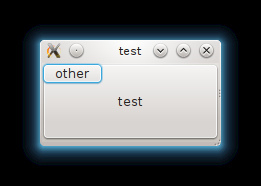
\includegraphics[width=0.3\textwidth]{./img/qt-usage-example.png}
  \caption{Usage example of Qt(withdrawn from~\cite{qt-usage})}%
\label{fig:qt-usage-example}
\end{figure}

The code that generates this \gls{ui} is the following:
%
\lstinputlisting[language=C++, firstline=1,
caption={Implementing a simple window in Qt},
label=lst:qt-usage-ex,
style= custom-cpp]{./listing/qt-usage-ex.cpp}
%

\subsubsection{Configuration with buildroot}
The configuration of Qt in buildroot to run on Raspberry Pi is pretty simple. 
In the $menuconfig$, it is just needed to select \texttt{Target packages}, then select \texttt{Graphic libraries and applications (graphic/text)} and finally select \texttt{Qt5}.

Then on the Qt5 menu select the following options presented on Fig.~\ref{fig:qt-buildroot}.
%
\begin{figure}[!hbt]
\centering
    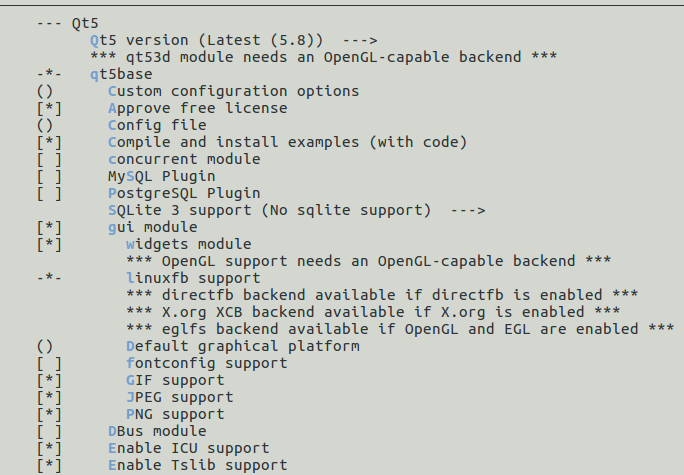
\includegraphics[width=0.6\textwidth]{./img/qt-buildroot.png}
  \caption{Selection of qt package in buildroot(withdrawn from~\cite{qt-root})}%
\label{fig:qt-buildroot}
\end{figure}

In conclusion, \texttt{Qt} is a great option to use on the project due to its features and also because it is very simple to use it on the project's board (Raspberry Pi).
%%% Local Variables:
%%% mode: latex
%%% TeX-master: "../../../dissertation"
%%% End:

% cli-serv
%
\section{File transfer protocols}
\label{sec:file-transf-prot}
Sometimes during the operation of all the system, it is necessary to transfer file between machines, for example, when a brand wants to upload video advertisements to its rent, or even when the admin wants to download that ad to verify its reliability.

\subsection{Protocols Overview}
\label{sub-sec:prot-overview}

There are various file transfer protocols to use, with different features and types of security and reliability. Throughout this various protocols, these are the most common ones~\cite{file-transf-protoc}:
%
\begin{item-c}
\item \emph{FTP}: it is a popular file transfer method that has been around for decades. FTP exchanges data using two separate channels known as the \texttt{command channel} to authenticate the user, and the \texttt{data channel} to transfer the files.
With FTP, both channels are \texttt{unencrypted}, leaving any data sent over these channels vulnerable to being taken advantage of. However, it does require an authenticated username and password for access.
%
\item \emph{FTPS}: it is a secure file transfer protocol that allows you to transfer files securely with trading partners, customers, and users. The transfers can be authenticated through FTPS-supported methods like client certificates, server certificates, and passwords.
%
\item \emph{SFTP}: it is a secure FTP protocol and a great alternative to unsecure FTP tools or manual scripts. SFTP exchanges data over an SSH connection and provides organizations with a high level of protection for file transfers shared between their systems, trading partners, employees, and the cloud.
%
\item \emph{SCP}: it is a network protocol that supports file transfers between hosts on a computer network. It's somewhat similar to FTP, however, SCP supports encryption and authentication features.
%
\item \emph{HTTP}: it is the foundation of data communication. It defines the format of messages through which web browsers and web servers communicate and defines how a web browser should response to a web request. HTTP uses \gls{tcp} as an underlying transport and is a stateless protocol. This means each command is executed independently and no session information is retained by the receiver.
%
\item \emph{HTTPS}: it is the secure version of HTTP where communications are encrypted by TLS or SSL.
\end{item-c}

\subsection{Which protocol is more efficient?}
\label{sub-sec:prot-effic}

In this case, \texttt{security} is one of the main goals, which means that all data must be sent in the best secure way possible. Thus, all file transfers must have \texttt{authentications} and \texttt{encryption}.
%
In conclusion, the better choice to this system is to chose the \texttt{HTTPS} protocol for several reasons:
\begin{item-c}
\item The communications between subsystems are made through \gls{tcp}/\gls{ip}, this is also used in this protocol, which is an advantage;
\item The data is transferred only with authentications (request and responses) which makes it more secure;
\item all communication is encrypted, which makes it even more secure.
\end{item-c} 

\subsection{Example of how to transfer files}
\label{sub-sec:file-transf-ex}

Here are examples on how to configure a connection fot file transfers and also how to download a file from a remote server using HTTPS.

\subsubsection{Configuring HTTP Connection Characteristics for File Transfers}
The following task is used to customize the connection characteristics for your network to specify a username and password, connection preferences, a remote proxy server, and the source interface to be used. These are the summary steps (that are then explained on Fig.~\ref{fig:configure-http-1} and Fig.~\ref{fig:configure-http-2})~\cite{http-example-cisco}:
%
\begin{enum-c}
\item enable;
\item configure terminal;
\item ip http client connection {forceclose | idletimeout <\texttt{seconds}> | timeout <\texttt{seconds}>};
\item ip http client username <\texttt{username}>;
\item ip http client password <\texttt{password}>;
\item ip http client proxy-server {<\texttt{proxy-name}> | <\texttt{ip-address}} [proxy-port <\texttt{port-number}>];
\item ip http client source-interface <\texttt{interface-id}>;
\item do copy running-config startup-config;
\item end.
\end{enum-c}
%
\begin{figure}[!hbt]
\centering
    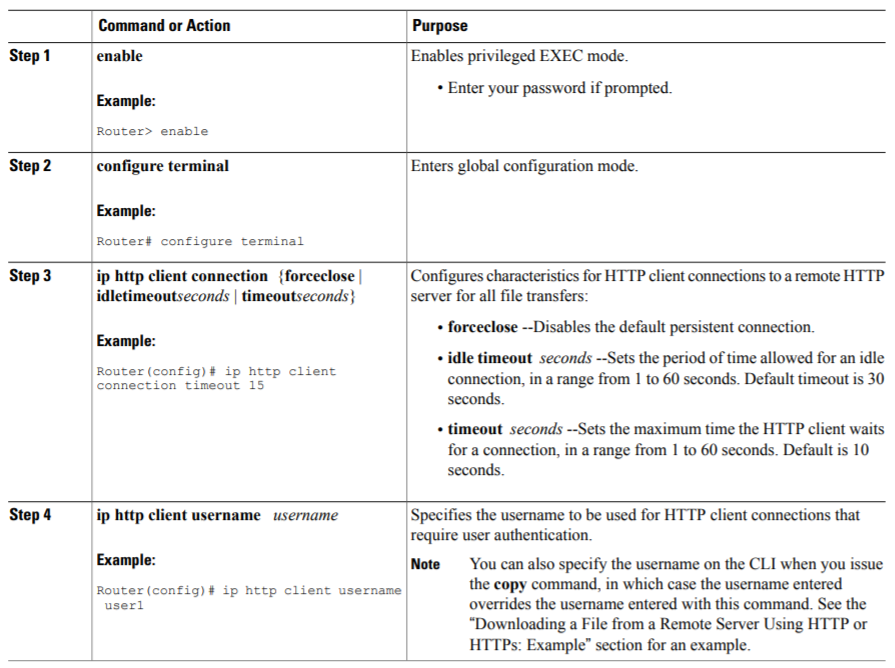
\includegraphics[width=0.8\textwidth]{./img/configure-http-1.png}
  \caption{Configuring HTTP Connection - 1(withdrawn from~\cite{http-example-cisco})}%
\label{fig:configure-http-1}
\end{figure}
%
\begin{figure}[!hbt]
\centering
    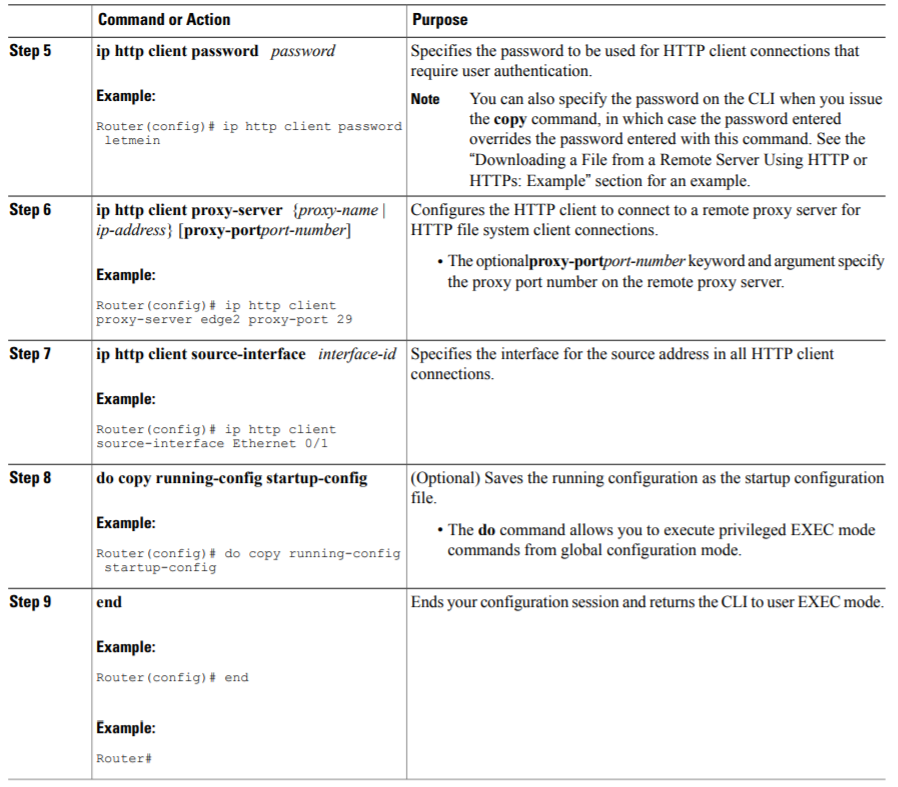
\includegraphics[width=0.8\textwidth]{./img/configure-http-2.png}
  \caption{Configuring HTTP Connection - 2(withdrawn from~\cite{http-example-cisco})}%
\label{fig:configure-http-2}
\end{figure}
%
\subsubsection{Downloading a File from a Remote Server Using HTTP or HTTPS}
Perform this task to download a file from a remote HTTP server using HTTP or HTTPs. The copy command helps you to copy any file from a source to a destination. These are the summary steps (that are then explained on Fig.~\ref{fig:download-http-1} and Fig.~\ref{fig:download-http-2})~\cite{http-example-cisco}:
%
\begin{enum-c}
\item enable;
\item Do one of the following:
	\begin{item-c}
	\item copy [/erase] [/noverify] http://<\texttt{remote-source-urllocal-destination-url}>;
	\item copy https:// <\texttt{remote-source-url local-destination-url}>.
	\end{item-c}
\end{enum-c}
%
\begin{figure}[!hbt]
\centering
    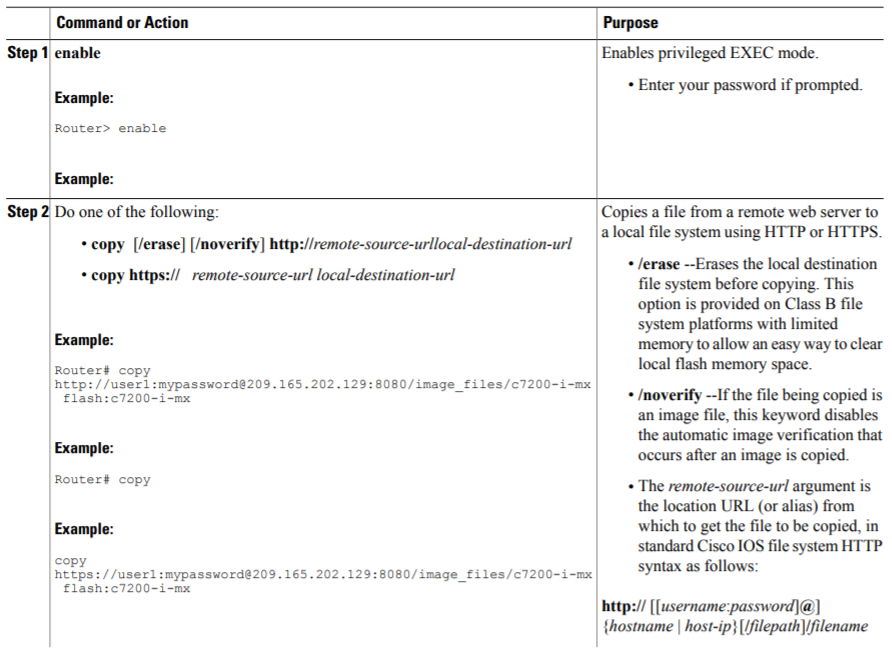
\includegraphics[width=0.8\textwidth]{./img/download-http-1.png}
  \caption{Downloading a File using HTTP - 1(withdrawn from~\cite{http-example-cisco})}%
\label{fig:download-http-1}
\end{figure}
%
\begin{figure}[!hbt]
\centering
    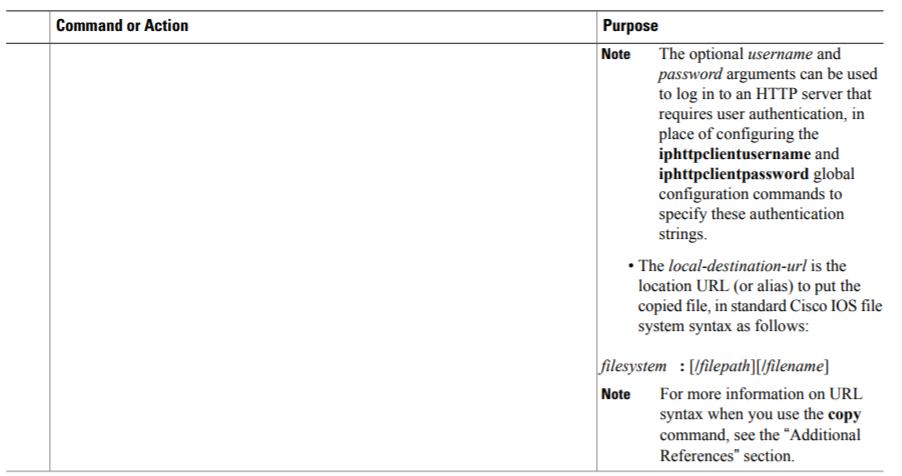
\includegraphics[width=0.8\textwidth]{./img/download-http-2.png}
  \caption{Downloading a File using HTTP - 2(withdrawn from~\cite{http-example-cisco})}%
\label{fig:download-http-2}
\end{figure}

\subsection{File Transfer Protocol \gls{api}s}
\label{sub-sec:ftp-apis}
There are several \gls{api}s that allow to develop applications in order to transfer files between two distinct points using file transfer protocols. The most common is \texttt{libcurl}, however, this is used in C language and it is necessary to use a wrapper to follow /gls{oop} paradigm, as it was previously said on subsection \ref{sec:c++-libraries-apis}.

In this case, it will be used one of the wrappers previously mentioned \texttt{curlpp}.

In Listing \ref{lst:http-post-ex} is an example on how does an HTTP POST is done. Basically it is crated an \texttt{easy} object that will handle all the POST request, inserting the \gls{url}, the header and the POST's field and size, then it is just needed to perform the request.
%
\lstinputlisting[language=C++, firstline=1,
caption={POST example using <curlpp.h>},
label=lst:http-post-ex,
style= custom-cpp]{./listing/http-post-ex.cpp}

\subsubsection{Third-party applications}

To make the file transfer more easier, it will be used a third-party application named \texttt{transfer.sh}. This application has easy-to-use commands in order to transfer files with a \gls{url}, there is unlimited upload, it can encrypt files and it is also possible to limit the amount of downloads and days available of downloading~\cite{transfer-sh}.

With a simple command like \texttt{curl --upload-file <path-to-the-file> https://transfer.sh/<name-that-you-want>} the file is uploaded to the site and it generates a \gls{url} to transfer that file using the command \texttt{curl <generated-url> -o <name-you-want>}.
And with this simple steps it is possible to easily transfer files between two nodes.

Using the library \texttt{curlpp} with the \texttt{transfer.sh} \gls{api}, it is possible to create a program to transfer files between nodes automatically when requested from the user, without the user needs to decorate or do such commands.
%
%%% Local Variables:
%%% mode: latex
%%% TeX-master: "../../../dissertation"
%%% End:

%
%%% Local Variables:
%%% mode: latex
%%% TeX-master: "../../../dissertation"
%%% End:
